%% PNAStwoS.tex
%% Sample file to use for PNAS articles prepared in LaTeX
%% For two column PNAS articles
%% Version1: Apr 15, 2008
%% Version2: Oct 04, 2013
\bibliographystyle{pnas}
%% BASIC CLASS FILE
\documentclass{pnastwo}

%% ADDITIONAL OPTIONAL STYLE FILES Font specification

%\usepackage{pnastwoF}


\usepackage{amsmath}
%% OPTIONAL MACRO DEFINITIONS
\def\s{\sigma}
%%%%%%%%%%%%
%% For PNAS Only:
\url{www.pnas.org/...}
\copyrightyear{20XX}
\issuedate{Issue Date}
\volume{Volume}
\issuenumber{Issue Number}
%\setcounter{page}{2687} %Set page number here if desired
%%%%%%%%%%%%

\begin{document}

\title{Sperm should evolve to make female meiosis fair}

\author{Yaniv Brandvain\affil{1}{Department of Plant Biology. University of Minnesota -- Twin Cities, St. Paul, MN, USA},
\and Graham Cooop\affil{2}{Department of Ecology and Evolution. University of California -- Davis. Davis, CA, USA}
}

\contributor{Submitted to Proceedings of the National Academy of Sciences
of the United States of America}

%%%Newly updated.
%%% If significance statement need, then can use the below command otherwise just delete it.
\significancetext{Female meiosis is the time during development where an allele can act to directly modify its representation in the next generation. 
The potential benefits to an allele that succeeds in this competition and collateral damage to organismal fitness are thought to have shaped basic features of female reproduction. 
However, little attention has been directed at the odd fact that fertilization by sperm is required to complete female meiosis in many species of animal. 
At first sight this seems strange as it seems to presents a dangerous opportunity for selfish alleles in sperm to distort the outcome of female meiosis in their own favor creating the opportunity for conflicts between male and female genomes. 
In this paper, through mathematical modeling, we show that in fact quite the opposite is true, sperm are usually selected to ensure the fairness of meiosis. 
Intuitively this comes about because selfish sperm have to immediately suffer any ill consequences of their actions in the resulting zygote, and so it is strongly in sperm's interests to keep genomes from gaming female meiosis. 
We hypothesize that the wide-spread requirement of fertilization to complete female meiosis may represent a long-term collaboration between male and female gametes to ensure fairness and the production of high quality gametes.}

\maketitle

\begin{article}
\begin{abstract}
{Genomic conflicts arise when an allele gains an evolutionary advantage at a cost to organismal fitness. 
%Because only one of four products of female meiosis is transmitted to offspring, 
O\"{o}genesis is inherently susceptible to such conflicts
because alleles compete to be the  product of female meiosis transmitted to the egg. 
Alleles that distort meiosis in their favor (i.e. meiotic drivers) often decrease organismal fitness,
	and therefore indirectly favor the evolution of mechanisms to suppress meiotic drive. In this light, many facets of  o\"{o}genesis and gametogenesis have been 
	interpreted as mechanisms of protection against genomic outlaws. 
Why then is female meiosis often left uncompleted until after
fertilization in many animals -- 
	potentially providing an opportunity for sperm alleles to
        meddle with its outcome and help like-alleles drive in heterozygous females? 
The population genetic theory presented herein suggests that
	sperm nearly always evolve to increase the fairness of female
        meiosis in the face of genomic conflicts.
These results are consistent with current knowledge of sperm-dependent meiotic drivers 
(loci whose distortion of female meiosis depends on sperm genotype),
	and suggest that the requirement of fertilization for the
        completion of female meiosis
        potentially represents a mechanism employed by females 
	 to ensure a fair meiosis.}
\end{abstract}

\keywords{meiosis | genomic conflict | meiotic drive | fertilization}



\dropcap{D}espite the apparent unity of the organism, `selfish' alleles can
gain an evolutionary advantage at a cost to  individual fitness
\cite{Burt2006}, often by exploiting meiosis and gametogenesis.
Because only one of the four products of female meiosis is transmitted to the egg, female meiosis is particularly vulnerable to such exploitation \cite{Sandler1957,Pardo-ManuelDeVillena2001a}. 
An allele that biases female meiosis in its favor (i.e. a meiotic driver), may increase in frequency even if it entails a pleiotropic fitness cost \cite{Prout1973}, generating a genetic conflict between the success of the driver and organismal fitness.
Meiotic drivers observed in both plants
\cite{Buckler1999,Fishman2005,Fishman2008}, and animals
\cite{Agulnik1990,Wu2005,Pardo-ManuelDeVillena2001c} highlight this
conflict -- the selfish benefits and the associated
pleiotropic fitness costs of drive sustain a balanced polymorphism
\cite{Prout1973}, 
and often generate ongoing evolutionary escalations of drive suppressors and enhancers \cite{Dawe1996,Fishman2008}. 
The threat of meiotic drive to organismal fitness is potentially so
severe that many basic properties of
meiosis and o\"{o}genesis, including the initial genome doubling in
meiosis I \cite{Haig1991}, arrested female meiosis
\cite{Mira1998}, the structure of centromere machinery \cite{Malik2002a,Malik2009}, and sex differences in the recombination rate \cite{Haig2010,Brandvain2012} 
have perhaps evolved to enforce fairness by disrupting meiotic drive \cite{Rice2013}.




It is therefore somewhat surprising that despite the intense evolutionary pressure on female meiosis to prevent meiotic drive, 
it is potentially open to sabotage by a virtual stranger -- a haploid sperm genome.
That is, in many animal species, female meiosis is completed only after fertilization \cite{Masui_book}, 
	creating ample opportunity for interaction between the sperm and
	female meiotic machinery (note that the alternation of generations in
	likely precludes this interaction in plants). 
Therefore, a `green-bearded' \cite{Gardner2010} sperm-acting allele that recognizes and facilitates the meiotic drive of a genetically equivalent allele in heterozygous females 
     could presumably rapidly spread through a population. 
At first sight, female meiosis appears primed for exploitation by such selfish systems.  
Why then is the requirement of fertilization to complete female meiosis so ubiquitous? 

It is certainly not the case that animals are mechanistically incapable of circumventing this requirement.
The stage at which female meiosis requires fertilization varies widely across taxa, and in a few animals  
	female meiosis is complete upon ovulation (that is, fertilization is not required for female meiosis (e.g. Table 1 in \cite {Masui_book}). 

It is also not the case that sperm is mechanistically incapable of influencing female meiosis.
In \emph{C. elegans}, premature deployment of the aster, a vital component of mitotic
machinery provided by the sperm, disrupts MII meiotic segregation
in the egg, leading to a triploid zygote \cite{McNally2012}. 
Thus, there is direct mechanistic evidence that sperm can influence female meiosis.
 Additionally, genetic evidence from the \emph{In} and \emph{Om}  drive systems in mice suggests that the 
 transmission of alternate alleles in heterozygous females can depend on sperm haplotype.  
 While ruling out the alternative hypothesis of early selection on zygotes in these cases is challenging (see pages 52-54 in \cite{Burt2006}), it appears that the extent to which \emph{In} and \emph{Om} distort the second female meiotic division partially depends on the genotype of the fertilizing sperm \cite{Agulnik1993,Wu2005}.  


We develop population genetic models exploring the evolution of sperm influence on female meiotic drive. 
We first focus on models in which `self-promoting' alleles in
  sperm facilitate drive of like alleles during gametogenesis in heterozygous females. 
These models show that such sperm-acting alleles 
	have more difficulty invading a population than do traditional meiotic drivers, 
	 and under most circumstances, cannot be maintained as a balanced polymorphism.
Because self-promoting drivers are unlikely to create a sustained genomic conflict, 
	female meiosis will have little incentive to evolve resistance to them.
We then examine models in which a novel sperm-acting allele modifies the efficacy of a polymorphic meiotic driver. 
Such model universally reveal that sperm-acting drive modifiers are favored only if the suppress drive. 
These results highlight the fact that the interests of sperm and maternal  genomes' are often aligned, as both are invested in the fate of the resultant zygote (as was speculated for the \emph{In} locus \cite{Pomiankowski1993}).
Therefore, there is little selective benefit to females in preventing sperm to influence female meioses.
Rather, features of o\"{o}genesis  may evolve to facilitate an interaction with sperm
	as yet another mechanism to enforce an equitable transfer of genetic material.


\section{Results}
\subsection{Invasion of an allele that promotes its own drive}
In the standard single-locus, biallelic model of female meiotic drive,
the driving allele is transmitted to the egg in heterozygotes with
probability  $d > 1/2$, regardless of sperm genotype (e.g. \cite{Ubeda2004} and see Model 1 in the Appendix for more details). 
To depict a case of a self-promoting meiotic driver,  we modify this standard model such 
	that the driver is only effective when fertilized by a sperm carrying that allele (see Figure 1A and Model 2 	in the Appendix and Table S1). 
We then identify the conditions allowing for the spread of this self-promoting driver, 
	and evaluate whether a driver of this form could generate a sustained conflict favoring the evolution of suppressors. 
We conclude our single locus results with an analysis of a related model (Model 3) - in which
drivers influence their transmission in females via paternal genotype,
rather than sperm haplotype. 

For comparative purposes, we first briefly present the standard drive model 
	(see e.g. \cite{Prout1973,Ubeda2004} for additional results). 
Assuming the driving allele is deleterious in both sexes, but fully recessive 
	(i.e. the fitness of drive homozygotes equals $w_{BB}=1-s$ and other genotypic fitnesses equal $w_{AA}=w_{AB}=1$), 
	it always invades because, when rare, it occurs predominantly in heterozygotes and therefore drives without a fitness cost. 
However, when $s$ is large ($s>(2d-1)/(2)$, solid black line in Figure 1B), a driver cannot fix, and
will be maintained as a protected polymorphism \cite{Prout1973}. 
The parameter space where the allele can invade but not fix is shown in white
        in Figure 1B. . 
When the allele is maintained as a polymorphism, it provides an opportunity for the evolution of
	drive suppressors, corresponding well to empirical examples of
        female meiotic drive (reviewed in \cite{Burt2006}). 

In contrast to a traditional driver, which drives but pays effectively
	no fitness cost when rare, 
a self-promoting driver specifically creates low fitness drive homozygotes 
	by uniting driving female gametes with sperm enabling that drive.
It must therefore overcome a drive-associated homozygous fitness cost simply to spread when rare. 
The conditions allowing the invasion of a self-promoting driver
 	are consequently far more restrictive than those for a standard meiotic driver.
When rare, a fully recessive, self-promoting driver can only invade when $s$ 
	is approximately less than $(2 d - 1)/(4 d)$ -- see dashed black line in Figure 1B. 
This analytical approximation, derived from Equation \eqref{deltadriver} assuming Hardy-Weinberg, 
	closely matches results obtained by exact numerical iteration (Figure 1B). 



When a self-promoting driver does spread, 
	it spends much time at low frequency, 
	because the paucity of complimentary sperm compromises its ability to drive. 
However, once relatively common, it  rapidly achieves fixation due to its
	positive frequency dependent behavior (Figure 1B.1).  
The positive frequency dependence of a self-promoting driver can also
	induce bistability in its spread -- some values of $s$ 
	allow the fixation of this driver when common, but 
	preclude its invasion when rare (Equation \ref{ineqA} and Figure 1B). 
In this case, the driver will be fixed if it reaches a frequency greater than some threshold 
	(approximated in Equation \ref{bistab_homozy_approx} and  presented exactly in 
	Figure S1), and lost otherwise. 
For most parameters, this threshold is likely too high to be reached by drift, 
	and therefore  the fate of self-promoting drivers is determined
	by the more restrictive invasion criteria rather than the fixation criteria. 

Inclusion of a heterozygous fitness cost (i.e. $w_{AB}=1-s_h$)
	further constrains the evolution of a self-promoting driver. 
In fact, with any heterozygous fitness cost, a rare self-promoting
	driver is always selected against. 
However, this case also displays bistability -- 
	when $s$ is sufficiently small (Equation \ref{sForHetFix}) this allele fixes deterministically if its 
	frequency exceeds some threshold  (Equation \ref{thresh2}, exact results in 
	Figure S2).

This bistability prevents self-promoting drivers from invading 	
	reasonably sized populations, and assures that if they do invade, they will rapidly fix.
Our model therefore predicts that self-promoting drivers will not be
	observed as stable polymorphisms in natural populations. 
This lack of a balanced polymorphism
	precludes the evolution of an
	allele that suppresses this form of meiotic drive in females.

Although the allelic identity of sperm could plausibly influence the outcome of female meiosis, 
	limited gene expression in sperm (e.g. \cite{Joseph2004}) 
	suggests a model where sperm influence female meiosis via expression of the fertilizing male's
	diploid genotype (perhaps due to proteins and RNAs packaged into the sperm), rather than sperm haplotype.
This paternal-genotype dependent model (Model 3  in the Appendix) requires one additional parameter, as we exchange $d$ in the sperm dependent case for $d_{het}$ and $d_{hom}$ which describe the transmission of the drive allele in a heterozygous female mating with males heterozygous and homozygous for the self-promoting drive allele, respectively.  
Here, a rare driver invades when $s$ is less than $(d_{het}-1/2)/d_{het}$, and usually fixes when it invades.
However, when the distorting effect of genotype displays strong dominance in its
	effect on female meiosis ($d_{het}$ is close to $d_{hom}$), 
	there is a a narrow sliver of parameter space sustains a polymorphism
	when the cost of the drive is recessive
	(see Figure S3, and Equation \ref{polymale}).  
While mathematically interesting, it does not seem particularly realistic to think that the
	effect of the drive allele would be dominant in its action through the
	male genotype, while the cost would be recessive. 
Therefore, although Model 3 can sustain a polymorphism, 
	the lack of biological reality underlying the small portion of parameter values 
	required for this polymorphism make us doubt it general applicability. 


Given the difficulty that self-promoting meiotic drivers have entering the population, the speed at
which they fix if they do, and the narrow parameter range permitting balanced polymorphisms at such loci,  
it seems very unlikely that such alleles could drive the evolution of female suppressors of sperm-enabled
female meiotic drive.

\subsection{Two locus models of sperm-dependent female drive}
Models 2 and 3, above, explored the dynamics of an allele that drove in females when signaled by a complementary signal in sperm.   
We complement this single-locus approach 
	with alternative models of two loci - one a female driver, 
	and the other, a sperm-acting allele which modifies the effect of drive upon fertilization. 
In this model, a female meiotic driver with no sperm-dependency 
	initially reaches drive-viability equilibrium (with two alleles
	$A$ and $B$ are the ancestral non-driver and driver alleles, Figure 2A1). 
Subsequently, a sperm-acting modifier of female meiotic drive arises at another locus. 

We first assume that the modifier is tightly
        linked to the drive locus (effectively creating a third
        allele/haplotype at this locus) and arises on the drive-background. 
Tight linkage offers the best
        chance for a collaboration to evolve between a driver and
       a sperm-acting drive  enhancer, as recombination breaks up drive haplotypes \cite{Thomson1974,Charlesworth1978,Haig1991}. 
Additionally, tight linkage between female driver and sperm modifier is consistent with the nature of well characterized drive systems which are often maintained as polymorphic inversions with numerous linked modifiers \cite{Burt2006}. 
We conclude by analyzing models with alternative linkage relationship between driver and drive modifier - 
	in Model 5 the modifier arises tightly linked to the non-driving allele, 
	and in Model 6 it is unlinked to the driver. 


%%%sperm-acting facilitator
When the modifier of drive is tightly linked to the driver and
enhances drive (i.e. in coupling phase), 
	we label  this non-recombining drive/modifier haplotype as the $B^+$ allele.  
The $B^+$ allele acts in sperm to increase the effectiveness of drive for both
	the $B$ and  $B^{+}$ alleles in $AB$ and $AB^{+}$ heterozygotes (see Figure 2A2, and Model 4 in the Appendix and Table S1). 
Naively, $B^{+}$ may spread by capitalizing on the additional drive it causes; however,  
	this is not the case for a few simple reasons. 
First, the novel $B^{+}$ haplotype
	arises when the ancestral driver 
	is at drive-selection balance, 
	and therefore immediately suffers a homozygous fitness cost.  
Worse yet, a novel $B^{+}$ haplotype most often helps 
	the $B$  allele drive ($B^+$ sperm meeting $AB$ eggs), because $B$ is initially more common than $B^{+}$. 
Therefore, sperm-acting drive facilitator alleles experience a profound disadvantage 
	in this scenario, even more so than under the previous two allele model. 
We have found no parameter range of this
	three allele system that allows the sperm-acting drive facilitator $B^{+}$ to
	invade the population (Appendix Model 4, Equation \eqref{coupling}, and Appendix S1). 

While  sperm enhancement of a female drive cannot displace a polymorphic female driver, sperm based drive suppressors can. 
Imagine a sperm-acting allele that restores fairness to female meiosis arises on
	the drive background, i.e. in repulsion phase, creating a
        third allele $B^{-}$, (Figure 2A3, Model 4 in Appendix). 
 This new allele still
        experiences female drive when fertilized by A or B sperm, but 
       is does not drive when fertilized by another $B^{-}$ so it
       avoid the excess formation of low fitness homozygotes. This
     allows the $B^{-}$ to displace the ancestral driver (Figure
     2, Equation \ref{coupling}), 
	and often returns to a lower equilibrium frequency than the the $B$ allele, further decreasing the extent of drive in the population.  
If this sperm-acting drive suppressor arises on 
	the non-driving $A$ background (creating a third allele $A^{-}$, Model 5), 
	or is unlinked to the drive locus (Model 6), it readily invades a population segregating
	for the drive system (Equations \ref{A-} and \ref{unlinked}).  
This allele lowers the frequency of the original driver (perhaps to zero),
	and spreads to fixation if it does not carry strong fitness costs
	(Figure 2B2). 
This result is consistent with previous work showing that drive suppressors unlinked to, or in repulsion phase with drivers usually invade polymorphic drive systems (e.g. \cite{Brandvain2012}).  
Therefore, all two-locus models of sperm influence on female drive suggest that
	sperm will evolve to oppose female meiotic drive.	
	


\section*{Discussion}

Sexual reproduction is a high-stakes event that determines what gets transmitted to the next generation.  
As a consequence of this intense competition, alleles that gain a transmission advantage during reproduction 
	can succeed evolutionarily even if they lower organismal fitness. 
This generates numerous conflicts  \cite{Burt2006} including sexual conflicts between mates \cite{Arnqvist2005}, 
	and conflicts between alleles that are over-transmitted in meiosis and the organisms they injure while doing so. 
Such conflicts and their resolution likely play a major role in the structure and evolution of many basic biological processes \cite{Rice2013}.

It seems that allowing sperm to influence the outcome of female meiosis would generate a confluence of these potential conflicts -- 
	sperm could actually assist an allele that distorts female meiosis.
However, this is not the case.
We find that an allele which acts through sperm to distort female meiosis in its favor 
	can rarely spread through a population if it bears any cost. 
Additionally, when this self-promoting driver can spread, it can only rarely 
	be maintained as a protected polymorphism, and due to its positive frequency dependence,  
	it spends very little time at intermediate frequency.
As such, this type of exploitation cannot generate a sustained genetic conflict.
It is therefore unlikely
	that female oogenesis and meiosis will evolve to prevent their effect.  
This likely explains why females can delay the completion of meiosis until after fertilization 
	without risking exploitation by collaborations by female
        drivers and sperm alleles.


Why is it that an allele that biases female meiosis in its favor can generate a genetic conflict, but an allele in sperm that assists this female driver cannot? 
So long as the transmission advantage of female meiotic drive outweigh the organismal fitness cost to heterozygotes the female driver can spread when rare, and it increases in 		
	frequency until the fitness cost experienced when homozygous balances the transmission advantage.
By contrast, a sperm promoter of female drive is only effective when matched with a heterozygote female -- meaning that, when rare, this allele rarely enhances female drive. 
Even worse, when it does so it will preferentially find itself in a low fitness drive homozygote. 
Not only are drive-promoting sperm alleles unable to create a sustained genetic conflict, 
	but alleles in sperm with the opposite effect - that is those that prevent their own drive through female meiosis do maintain a polymorphism and 
	provide evolution  with time and opportunity to further minimize drive.
This is because such drive suppressing alleles reduced their chances
of forming low fitness homozygotes. 
More generally, alleles that act through sperm to
 reduce the opportunity of female meiotic drive regardless of linkage or phase. 
 
Our theory offers a novel interpretation of a baffling idiosyncrasy of female meiosis -- 
	we argue that females do not complete meiosis until after fertilization as a mechanism to encourage meiotic fairness. 
In addition to providing a new interpretation of a basic biological process, our theory provides numerous testable predictions. 
We predict that female drive, at a stage influenceable by sperm,  
	should be reduced when fertilized by
	complimentary sperm. 
Therefore, For example, MII female drive should be exceptionally severe in
	interspecific crosses between animals which complete the second meiotic division after fertilization,  
	as heterospecific sperm will not specifically evolve to resists a female driver in another species. 
Our theory also encourages phylogenetic hypotheses concerning the relationship between the opportunity 
	for female meiotic drive the requirement of fertilization for the completion of female meiosis. 
For example, we predict that a lower opportunity for female meiotic drive,
        e.g. an animal lineage with a long history of high inbreeding
        or selfing, 
        would often accompanied by a relaxation of the requirement of fertilization for the
        completion of female meiosis.


Our results highlight potentially counterintuitive results of complex genetic conflicts. 
Despite much opportunity for conflict between sperm and females over fertilization \cite{Partridge1998},
	the interests of fertilizing sperm and female are quite well aligned during syngamy.
While conflict between mother and her alternative chromosomes ensue, 
	fertilizing sperm decidedly side with mom, as both have a shared interest in producing a viable and potentially fit offspring. 


\section{Appendix}
We highlight simple analytical results from: 
	the standard model of female meiotic drive (Model 1); a sperm-dependent 
	model of female meiotic drive (Model 2); a male-genotype-dependent model of
	female meiotic drive (Model 3); and more complex two-locus sperm-dependent drive models (Models 4-6). 
All models include a biallelic locus ($A/B$) with non-driving and driving alleles in frequencies $f_A$ and $f_B$, 
	respectively, while more complex models include more loci and/or alleles.  
Transmission rules describing the outcomes of all matings in each
	model are presented in Table S1. 
The fitness of genotype, $g$ is sex-independent and equals $1$, $1-h_s$, and $1-s$ for genotypes $AA$, $AB$, and $BB$, respectively. 
Genotypic frequencies  equal  $f_g$ for adults in the current generation, 
	$f_g'$ in the next generation of zygotes (i.e. after recombination, random mating, drive, and syngamy, but before selection)
	and $f_g''$ in adults after selection. 
After a complete generation $f_g'' = f_g' w_g/\bar{w}$, where $\bar{w}$ is the population mean fitness and equals $\Sigma w_g f_g'$. 
Because many of our analyses assume genotype frequencies expected under Hardy Weinberg Equilibrium (HWE), we note which analytical results are approximations. 
We verify these approximations with exact numerical iterations in Figures S1-S3 , and detail the derivation of these approximations in Appendix S1.  



\subsection{Models 1-3. Single-locus drive}
\subsubsection{Model 1. Traditional driver:}
In the standard female drive model, meiosis in males is fair such that $A/B$ heterozygotes contribute $A$ and $B$ alleles with equal probabilities; however, $A/B$ females transmit the $B$ allele with probability $d>1/2$.  
We note that the timing of fertilization relative to female meiosis places another constraint on $d$, for example, if fertilization (and therefore, sperm dependent drive) takes place at MII (as in mammals),
	female drive requires an uneven number of crossovers between the centromere and the drive locus, 
	so $d$ is bounded to be $<0.83$ (see \cite{Buckler1999} for discussion). 
After drive and random mating, genotype frequencies are 
\begin{eqnarray*}
f_{AA}'&=&f_A (f_{AA }+ f_{AB} (1 - d)),\\
f_{AB}'&=&f_A (f_{BB} + f_{ABd}) + f_B (f_{AA} + f_{AB} (1 - d)),\\
f_{BB}'&=& f_B (f_{AB} d + f_{BB})
\end{eqnarray*}
As detailed above, exact frequencies after drive, random mating and selection are $f_g''= f_g'w_g/\bar{w}$. 
Assuming HWE, a rare driver will spread when $s_h
        \lessapprox(2d-1)/(1+2d)$, and will fix when $s\lessapprox d -1/2 +
        3 s_h /2- d s_h$. This later inequality reduces to
        $s\lessapprox(2d-1)/2$ when the cost of drive is fully
        recessive. 

\subsubsection{Model 2. Single locus, sperm-dependent drive:}
Our single-locus model of sperm-dependent drive resembles the traditional driver, with the caveat that the $B$ allele drives in heterozygous females only when fertilized by $B$-bearing sperm. 
Therefore, genotype frequencies after drive are 
\begin{eqnarray*}
f_{AA}'&=&f_A^2,\\
f_{AB}'&=&f_A f_B+f_B (f_{AA} + f_{AB}(1 - d)) ,\\
f_{BB}'&=&f_B (f_{AB} d + f_{BB} )
\end{eqnarray*}

We iterate exact genotype frequency recursions ($f_g''= f_g'w_g/\bar{w}$) over generations to produce the frequency trajectories shown in the inset of
Figure 1B by plotting $f_B=f_{BB}+ \frac{1}{2}f_{AB}$
over time. 
To assess invasion or fixation criteria, as well as bistability points, we iterate this system and
test whether $f_B$ increases over a grid of parameters. 

\paragraph{Recessive fitness cost of self-promoting driver -- }
When fully recessive, the change in frequency of the self-promoting driver across generations equals 
\begin{equation}
\Delta f_B=\frac{f_A f_B^2}{\bar{w}} \left( \left(1-F\right)\left( d\left(1-2 f_A s\right) - f_B s-\frac{1}{2}\right) - s  F \right)
\label{deltadriver}
\end{equation}
where $F$ is the deviation from genotypic frequencies expected under Hardy-Weinberg. 
Assuming HWE  ($F=0$) a common, recessive, self-promoting driver invades if $s\lessapprox(2 d - 1)/(4 d)$, and fixes if
 $s\lessapprox(2d-1)/2$. 
 Therefore, when 
\begin{equation}
(2 d - 1)/(4 d)  \lessapprox  s  \lessapprox  (2d-1)/2\label{ineqA}
\end{equation} 
a recessive, self-promoting driver will deterministically fix if drift,
 	mutation, or migration pressure bring its frequency above
\begin{equation} 
f^*_{B\text{ recessive}} \approx (1-2d+4ds)/(2s(2d-1)) \label{bistab_homozy_approx}
\end{equation}
 but it will be lost when introduced below this frequency. 
 Compared to exact results (Figure S1), Equations
 \eqref{ineqA} and \eqref{bistab_homozy_approx} offer reasonable, but imperfect approximations. 
 
 
 \paragraph{Cost of driver in heterozygotes -- } 
When the fitness of drive heterozygotes is compromised ($s_h>0$), a self-promoting driver cannot invade when rare.
This results from the fact that,
when rare, 
$B$-bearing sperm and heterozygous eggs will rarely encounter one another ($\sim f_B^2$) but the allele still pays a
cost in heterozygous individuals ($\sim f_B$). 
However, this system too, is bistable -- as the driver increases in frequency it is more often fertilized by a driving sperm and therefore drives more effectively. 
Therefore, assuming HWE, if 
\begin{equation}
	s \lessapprox  d -1/2 +s_h(3-2d)/2
	\label{sForHetFix}
\end{equation}
this self-promoting driver deterministically fixes when its frequency is greater than
\begin{equation}
	f_B^* \approx \frac{a_1+\sqrt{a_1^2+8 s_h a_2}}{2 a_2}
	\label{thresh2}
\end{equation}
where, $a_1=1-2 ds_h+4 d s-2 d-3 s_h$ and $a_2=2(s-s_h)(2d-1)$.
Comparison of Equation \ref{thresh2} to exact results obtained by a
simple parameter search (Figure S2)
show that this approximation is reasonably correct for small
parameter values; however, it underestimates $f_B^*$ for large parameter values, presumably because they result in strong departures from HWE.


\subsubsection{Model 3. Single locus, paternal genotype dependent drive:}
In the case when female meiotic drive depends on paternal genotype
 heterozygous female will transmit the $B$ allele 
  with probabilities  $\frac{1}{2}$,  $d_{het}\geq 1/2 $ or $d_{hom}\geq d_{het}$, 
 when mated with to $AA$, $AB$, or $BB$ males,  respectively. 
  In this model, genotype frequencies after drive, random mating, and selection are 
  
\begin{eqnarray*}
f_{AA}''&=&\frac{w_{AA}}{2\bar{w}}\left( f_{AA} (2 f_A + f_{AB} ) + f_{AB}^2 (1 - d_{het}) \right),\\
f_{AB}''&=&\frac{w_{AB}}{\bar{w}}\big(f_{AA} (f_B + f_{AB}/2) +  f_{AB} f_B \\&& + f_{BB}(f_A - f_{AB} d_{hom})\big),\\
f_{BB}''&=&\frac{w_{BB}}{\bar{w}}\left((f_{AB} (f_{AB} d_{het}/2 + f_{BB} d_{hom}) + f_{BB} f_B\right)
\end{eqnarray*}



If the cost of drive is fully recessive (i.e. $s_h=0$), assuming HWE, 
	a rare paternal-genotype-dependent driver invades when 
	$s\lessapprox (d_{het}-1/2)/(d_{het})$, and when common, this driver fixes if 
	$s\lessapprox d_{hom}-1/2$, approximations well supported by exact results (Figure S3).
Specifically, when drive in heterozygotes is large relative to that in homozygotes, 
	\begin{equation} d_{het}  \gtrapprox 1/(3-2d_{hom}) \label{polymale} \end{equation}
	fixation criteria are more stringent than invasion criteria, 
	and therefore some values of $s$ can maintain a stable polymorphism. 
Under these parameter values, a rare paternal-genotype-dependent driver 
	can increase in frequency because it gains a transmission advantage and suffers 
	no fitness cost when heterozygous eggs are fertilized by 
	$A$-bearing sperm of heterozygous males. 
As the frequency of the $B$ allele increases, 
	it will be unable to 
	avoid producing unfit homozygous offspring, leaving it trapped in
	the population at frequency $f_{B\text{ pat}}^*$. 
Assuming HWE, a recessive fitness cost ($h_s=0$), and dominance of driver ($d_{het}=d_{hom}$) this equilibrium frequency is
\begin{equation}f_{B\text{ pat}}^*\approx2 (1 + 2d_{hom}[s - 1])/([2 s - 1][2d_{hom}- 1]) \label{eqmale} \end{equation}
By contrast, when $d_{het} \lessapprox 1/(3-2d_{hom})$ the case is reversed, and the model is bistable.
 
 
 
\subsection{Models 4-6. Two-locus, sperm-dependent drive} 
Assuming that a traditional driver segregates at its equilibrium frequency (Model 1), we investigate the evolution of tightly linked (Models 4 and 5), and unlinked (Model 6) sperm-dependent modifiers of drive. 
In Models 4 and 5, we treat this two-locus system as if it consists of
a single locus with three alleles: $A$, $B$ and $C$, corresponding to the case when the
sperm-modifier arises once, tightly linked to one or other of the
alleles at the drive locus (such that recombination is unexpected). 
In all cases, we assume that fitness is independent of the drive modifier.  
We assume the traditional driver is transmitted to $d_0$ of gametes from female heterozygotes  when fertilized by wild-type sperm, and $d_1=d_0+\epsilon$ when fertilized by a sperm-acting drive-modifier.

\subsubsection*{Model 4. Drive-modifier in coupling phase:}
When the $C$ allele is tightly linked to the driver allele, 
	genotypic fitnesses equal $w_{AC}=w_{AB}=1-s_h$, and $w_{BC}=w_{CC}=w_{BB}=1-s$. 
Assuming HWE, a recessive fitness cost to drive, and assuming that the $A/B$ locus is at its equilibrium frequency, the change in frequency of a rare drive modifier is


\begin{eqnarray}\nonumber
\Delta C\approx -\epsilon \frac{f_C}{2 \bar{w}(1-2 d_0)^2} \bigg( 1-2 d_0 (-2 d_0+s+2) \\
 +\sqrt{2} \sqrt{s (2 d_0 (d_0(s-2)+2)-1)} \bigg)
	\label{coupling}
\end{eqnarray} 



For all parameters sustaining a polymorphism at the drive locus ($s>d_0-1/2$), this corresponds to a decrease in frequency of the $C$ allele when it enhances drive ($\epsilon >0$ -- the $B^+$ model, above), 
	and an increase in frequency of the $C$ allele when it suppresses drive ($\epsilon <0$ -- the $B^-$ model, above). 
More generally, even when the cost of drive is not fully recessive, the $B^-$ allele will invade and fix under all parameters sustaining a previous polymorphism at the drive locus (see Appendix S1). 
 
 \subsubsection{Model 5. Drive-modifier in repulsion phase:}
When the $C$ allele is tightly linked to the non-driver, 
	genotypic fitnesses equal $w_{CC}=w_{AC}=w_{AA}=1$, and $w_{BC}=w_{AB}=1-s_h$. 
Assuming HWE, a recessive fitness cost to drive, and assuming that the $A/B$ locus is at its equilibrium frequency, the change in frequency of a rare drive modifier is
\begin{equation}
	\Delta C \approx -\epsilon f_{C^-}^2 \frac{ \left(2 d_0 s-\sqrt{2} \\ \sqrt{s (2 d_0 (d_0 (s-2)+2)-1)}\right)}{2\bar{w}s (2 d_0 -1) } \label{A-}
\end{equation}
For all values of interest ($0<s<1$, $0.5<d_0<1$), the change in frequency a rare $C$ allele is positive when it decreases drive (i.e. $\epsilon <0$, corresponding to the $A^-$ model, above), a result which holds qualitatively for a common $C$ allele, as well (Appendix S1). 
Somewhat counterintuitively, the spread of the $A^-$ allele is substantially slower than that of the $B^-$ allele (it is on the order of $C^{2}$ rather than $C$). 
This is because the $A^-$ allele will never occur in drive-homozygotes and therefore only spreads by preventing itself from the cheating of the driver.

\subsubsection*{Model 6. Unlinked drive-modifier:}
For the unlinked model, we introduce another locus where drive is modified in $A/B$ females fertilized by $M$ allele, 
	while the wild-type $L$ allele does not influence drive. 
Assuming HWE and linkage equilibrium, the change in frequency of a rare unlinked, sperm-acting drive modifier is 
\begin{equation} \Delta M =-\epsilon f_A f_B (f_B s + s_h (f_A - f_B) ) \frac{f_M}{\bar{w}}  \label{unlinked} \end{equation}
Thus, a rare drive suppressor ($\epsilon<0$) will spread so long as the fitness cost of the driver does not display over- or under-dominance. 
Notably, this result holds while assuming complete linkage equilibrium, and therefore sperm suppression of female meiotic drive is likely more powerful than more direct female-enforced drive suppressors  which usually spread due to the indirect benefit of avoiding drive haplotypes (e.g. \cite{Brandvain2012}).  
 
\begin{acknowledgments} \end{acknowledgments}
%\bibliography{refs}
%% PNAStwoS.tex
%% Sample file to use for PNAS articles prepared in LaTeX
%% For two column PNAS articles
%% Version1: Apr 15, 2008
%% Version2: Oct 04, 2013
\bibliographystyle{pnas}
%% BASIC CLASS FILE
\documentclass{pnastwo}

%% ADDITIONAL OPTIONAL STYLE FILES Font specification

%\usepackage{pnastwoF}


\usepackage{amsmath}
%% OPTIONAL MACRO DEFINITIONS
\def\s{\sigma}
%%%%%%%%%%%%
%% For PNAS Only:
\url{www.pnas.org/...}
\copyrightyear{20XX}
\issuedate{Issue Date}
\volume{Volume}
\issuenumber{Issue Number}
%\setcounter{page}{2687} %Set page number here if desired
%%%%%%%%%%%%

\begin{document}

\title{Sperm should evolve to make female meiosis fair}

\author{Yaniv Brandvain\affil{1}{Department of Plant Biology. University of Minnesota -- Twin Cities, St. Paul, MN, USA},
\and Graham Cooop\affil{2}{Department of Ecology and Evolution. University of California -- Davis. Davis, CA, USA}
}

\contributor{Submitted to Proceedings of the National Academy of Sciences
of the United States of America}

%%%Newly updated.
%%% If significance statement need, then can use the below command otherwise just delete it.
\significancetext{Female meiosis is the time during development where an allele can act to directly modify its representation in the next generation. 
The potential benefits to an allele that succeeds in this competition and collateral damage to organismal fitness are thought to have shaped basic features of female reproduction. 
However, little attention has been directed at the odd fact that fertilization by sperm is required to complete female meiosis in many species of animal. 
At first sight this seems strange as it seems to presents a dangerous opportunity for selfish alleles in sperm to distort the outcome of female meiosis in their own favor creating the opportunity for conflicts between male and female genomes. 
In this paper, through mathematical modeling, we show that in fact quite the opposite is true, sperm are usually selected to ensure the fairness of meiosis. 
Intuitively this comes about because selfish sperm have to immediately suffer any ill consequences of their actions in the resulting zygote, and so it is strongly in sperm's interests to keep genomes from gaming female meiosis. 
We hypothesize that the wide-spread requirement of fertilization to complete female meiosis may represent a long-term collaboration between male and female gametes to ensure fairness and the production of high quality gametes.}

\maketitle

\begin{article}
\begin{abstract}
{Genomic conflicts arise when an allele gains an evolutionary advantage at a cost to organismal fitness. 
%Because only one of four products of female meiosis is transmitted to offspring, 
O\"{o}genesis is inherently susceptible to such conflicts
because alleles compete to be the  product of female meiosis transmitted to the egg. 
Alleles that distort meiosis in their favor (i.e. meiotic drivers) often decrease organismal fitness,
	and therefore indirectly favor the evolution of mechanisms to suppress meiotic drive. In this light, many facets of  o\"{o}genesis and gametogenesis have been 
	interpreted as mechanisms of protection against genomic outlaws. 
Why then is female meiosis often left uncompleted until after
fertilization in many animals -- 
	potentially providing an opportunity for sperm alleles to
        meddle with its outcome and help like-alleles drive in heterozygous females? 
The population genetic theory presented herein suggests that
	sperm nearly always evolve to increase the fairness of female
        meiosis in the face of genomic conflicts.
These results are consistent with current knowledge of sperm-dependent meiotic drivers 
(loci whose distortion of female meiosis depends on sperm genotype),
	and suggest that the requirement of fertilization for the
        completion of female meiosis
        potentially represents a mechanism employed by females 
	 to ensure a fair meiosis.}
\end{abstract}

\keywords{meiosis | genomic conflict | meiotic drive | fertilization}



\dropcap{D}espite the apparent unity of the organism, `selfish' alleles can
gain an evolutionary advantage at a cost to  individual fitness
\cite{Burt2006}, often by exploiting meiosis and gametogenesis.
Because only one of the four products of female meiosis is transmitted to the egg, female meiosis is particularly vulnerable to such exploitation \cite{Sandler1957,Pardo-ManuelDeVillena2001a}. 
An allele that biases female meiosis in its favor (i.e. a meiotic driver), may increase in frequency even if it entails a pleiotropic fitness cost \cite{Prout1973}, generating a genetic conflict between the success of the driver and organismal fitness.
Meiotic drivers observed in both plants
\cite{Buckler1999,Fishman2005,Fishman2008}, and animals
\cite{Agulnik1990,Wu2005,Pardo-ManuelDeVillena2001c} highlight this
conflict -- the selfish benefits and the associated
pleiotropic fitness costs of drive sustain a balanced polymorphism
\cite{Prout1973}, 
and often generate ongoing evolutionary escalations of drive suppressors and enhancers \cite{Dawe1996,Fishman2008}. 
The threat of meiotic drive to organismal fitness is potentially so
severe that many basic properties of
meiosis and o\"{o}genesis, including the initial genome doubling in
meiosis I \cite{Haig1991}, arrested female meiosis
\cite{Mira1998}, the structure of centromere machinery \cite{Malik2002a,Malik2009}, and sex differences in the recombination rate \cite{Haig2010,Brandvain2012} 
have perhaps evolved to enforce fairness by disrupting meiotic drive \cite{Rice2013}.




It is therefore somewhat surprising that despite the intense evolutionary pressure on female meiosis to prevent meiotic drive, 
it is potentially open to sabotage by a virtual stranger -- a haploid sperm genome.
That is, in many animal species, female meiosis is completed only after fertilization \cite{Masui_book}, 
	creating ample opportunity for interaction between the sperm and
	female meiotic machinery (note that the alternation of generations in
	likely precludes this interaction in plants). 
Therefore, a `green-bearded' \cite{Gardner2010} sperm-acting allele that recognizes and facilitates the meiotic drive of a genetically equivalent allele in heterozygous females 
     could presumably rapidly spread through a population. 
At first sight, female meiosis appears primed for exploitation by such selfish systems.  
Why then is the requirement of fertilization to complete female meiosis so ubiquitous? 

It is certainly not the case that animals are mechanistically incapable of circumventing this requirement.
The stage at which female meiosis requires fertilization varies widely across taxa, and in a few animals  
	female meiosis is complete upon ovulation (that is, fertilization is not required for female meiosis (e.g. Table 1 in \cite {Masui_book}). 

It is also not the case that sperm is mechanistically incapable of influencing female meiosis.
In \emph{C. elegans}, premature deployment of the aster, a vital component of mitotic
machinery provided by the sperm, disrupts MII meiotic segregation
in the egg, leading to a triploid zygote \cite{McNally2012}. 
Thus, there is direct mechanistic evidence that sperm can influence female meiosis.
 Additionally, genetic evidence from the \emph{In} and \emph{Om}  drive systems in mice suggests that the 
 transmission of alternate alleles in heterozygous females can depend on sperm haplotype.  
 While ruling out the alternative hypothesis of early selection on zygotes in these cases is challenging (see pages 52-54 in \cite{Burt2006}), it appears that the extent to which \emph{In} and \emph{Om} distort the second female meiotic division partially depends on the genotype of the fertilizing sperm \cite{Agulnik1993,Wu2005}.  


We develop population genetic models exploring the evolution of sperm influence on female meiotic drive. 
We first focus on models in which `self-promoting' alleles in
  sperm facilitate drive of like alleles during gametogenesis in heterozygous females. 
These models show that such sperm-acting alleles 
	have more difficulty invading a population than do traditional meiotic drivers, 
	 and under most circumstances, cannot be maintained as a balanced polymorphism.
Because self-promoting drivers are unlikely to create a sustained genomic conflict, 
	female meiosis will have little incentive to evolve resistance to them.
We then examine models in which a novel sperm-acting allele modifies the efficacy of a polymorphic meiotic driver. 
Such model universally reveal that sperm-acting drive modifiers are favored only if the suppress drive. 
These results highlight the fact that the interests of sperm and maternal  genomes' are often aligned, as both are invested in the fate of the resultant zygote (as was speculated for the \emph{In} locus \cite{Pomiankowski1993}).
Therefore, there is little selective benefit to females in preventing sperm to influence female meioses.
Rather, features of o\"{o}genesis  may evolve to facilitate an interaction with sperm
	as yet another mechanism to enforce an equitable transfer of genetic material.


\section{Results}
\subsection{Invasion of an allele that promotes its own drive}
In the standard single-locus, biallelic model of female meiotic drive,
the driving allele is transmitted to the egg in heterozygotes with
probability  $d > 1/2$, regardless of sperm genotype (e.g. \cite{Ubeda2004} and see Model 1 in the Appendix for more details). 
To depict a case of a self-promoting meiotic driver,  we modify this standard model such 
	that the driver is only effective when fertilized by a sperm carrying that allele (see Figure 1A and Model 2 	in the Appendix and Table S1). 
We then identify the conditions allowing for the spread of this self-promoting driver, 
	and evaluate whether a driver of this form could generate a sustained conflict favoring the evolution of suppressors. 
We conclude our single locus results with an analysis of a related model (Model 3) - in which
drivers influence their transmission in females via paternal genotype,
rather than sperm haplotype. 

For comparative purposes, we first briefly present the standard drive model 
	(see e.g. \cite{Prout1973,Ubeda2004} for additional results). 
Assuming the driving allele is deleterious in both sexes, but fully recessive 
	(i.e. the fitness of drive homozygotes equals $w_{BB}=1-s$ and other genotypic fitnesses equal $w_{AA}=w_{AB}=1$), 
	it always invades because, when rare, it occurs predominantly in heterozygotes and therefore drives without a fitness cost. 
However, when $s$ is large ($s>(2d-1)/(2)$, solid black line in Figure 1B), a driver cannot fix, and
will be maintained as a protected polymorphism \cite{Prout1973}. 
The parameter space where the allele can invade but not fix is shown in white
        in Figure 1B. . 
When the allele is maintained as a polymorphism, it provides an opportunity for the evolution of
	drive suppressors, corresponding well to empirical examples of
        female meiotic drive (reviewed in \cite{Burt2006}). 

In contrast to a traditional driver, which drives but pays effectively
	no fitness cost when rare, 
a self-promoting driver specifically creates low fitness drive homozygotes 
	by uniting driving female gametes with sperm enabling that drive.
It must therefore overcome a drive-associated homozygous fitness cost simply to spread when rare. 
The conditions allowing the invasion of a self-promoting driver
 	are consequently far more restrictive than those for a standard meiotic driver.
When rare, a fully recessive, self-promoting driver can only invade when $s$ 
	is approximately less than $(2 d - 1)/(4 d)$ -- see dashed black line in Figure 1B. 
This analytical approximation, derived from Equation \eqref{deltadriver} assuming Hardy-Weinberg, 
	closely matches results obtained by exact numerical iteration (Figure 1B). 



When a self-promoting driver does spread, 
	it spends much time at low frequency, 
	because the paucity of complimentary sperm compromises its ability to drive. 
However, once relatively common, it  rapidly achieves fixation due to its
	positive frequency dependent behavior (Figure 1B.1).  
The positive frequency dependence of a self-promoting driver can also
	induce bistability in its spread -- some values of $s$ 
	allow the fixation of this driver when common, but 
	preclude its invasion when rare (Equation \ref{ineqA} and Figure 1B). 
In this case, the driver will be fixed if it reaches a frequency greater than some threshold 
	(approximated in Equation \ref{bistab_homozy_approx} and  presented exactly in 
	Figure S1), and lost otherwise. 
For most parameters, this threshold is likely too high to be reached by drift, 
	and therefore  the fate of self-promoting drivers is determined
	by the more restrictive invasion criteria rather than the fixation criteria. 

Inclusion of a heterozygous fitness cost (i.e. $w_{AB}=1-s_h$)
	further constrains the evolution of a self-promoting driver. 
In fact, with any heterozygous fitness cost, a rare self-promoting
	driver is always selected against. 
However, this case also displays bistability -- 
	when $s$ is sufficiently small (Equation \ref{sForHetFix}) this allele fixes deterministically if its 
	frequency exceeds some threshold  (Equation \ref{thresh2}, exact results in 
	Figure S2).

This bistability prevents self-promoting drivers from invading 	
	reasonably sized populations, and assures that if they do invade, they will rapidly fix.
Our model therefore predicts that self-promoting drivers will not be
	observed as stable polymorphisms in natural populations. 
This lack of a balanced polymorphism
	precludes the evolution of an
	allele that suppresses this form of meiotic drive in females.

Although the allelic identity of sperm could plausibly influence the outcome of female meiosis, 
	limited gene expression in sperm (e.g. \cite{Joseph2004}) 
	suggests a model where sperm influence female meiosis via expression of the fertilizing male's
	diploid genotype (perhaps due to proteins and RNAs packaged into the sperm), rather than sperm haplotype.
This paternal-genotype dependent model (Model 3  in the Appendix) requires one additional parameter, as we exchange $d$ in the sperm dependent case for $d_{het}$ and $d_{hom}$ which describe the transmission of the drive allele in a heterozygous female mating with males heterozygous and homozygous for the self-promoting drive allele, respectively.  
Here, a rare driver invades when $s$ is less than $(d_{het}-1/2)/d_{het}$, and usually fixes when it invades.
However, when the distorting effect of genotype displays strong dominance in its
	effect on female meiosis ($d_{het}$ is close to $d_{hom}$), 
	there is a a narrow sliver of parameter space sustains a polymorphism
	when the cost of the drive is recessive
	(see Figure S3, and Equation \ref{polymale}).  
While mathematically interesting, it does not seem particularly realistic to think that the
	effect of the drive allele would be dominant in its action through the
	male genotype, while the cost would be recessive. 
Therefore, although Model 3 can sustain a polymorphism, 
	the lack of biological reality underlying the small portion of parameter values 
	required for this polymorphism make us doubt it general applicability. 


Given the difficulty that self-promoting meiotic drivers have entering the population, the speed at
which they fix if they do, and the narrow parameter range permitting balanced polymorphisms at such loci,  
it seems very unlikely that such alleles could drive the evolution of female suppressors of sperm-enabled
female meiotic drive.

\subsection{Two locus models of sperm-dependent female drive}
Models 2 and 3, above, explored the dynamics of an allele that drove in females when signaled by a complementary signal in sperm.   
We complement this single-locus approach 
	with alternative models of two loci - one a female driver, 
	and the other, a sperm-acting allele which modifies the effect of drive upon fertilization. 
In this model, a female meiotic driver with no sperm-dependency 
	initially reaches drive-viability equilibrium (with two alleles
	$A$ and $B$ are the ancestral non-driver and driver alleles, Figure 2A1). 
Subsequently, a sperm-acting modifier of female meiotic drive arises at another locus. 

We first assume that the modifier is tightly
        linked to the drive locus (effectively creating a third
        allele/haplotype at this locus) and arises on the drive-background. 
Tight linkage offers the best
        chance for a collaboration to evolve between a driver and
       a sperm-acting drive  enhancer, as recombination breaks up drive haplotypes \cite{Thomson1974,Charlesworth1978,Haig1991}. 
Additionally, tight linkage between female driver and sperm modifier is consistent with the nature of well characterized drive systems which are often maintained as polymorphic inversions with numerous linked modifiers \cite{Burt2006}. 
We conclude by analyzing models with alternative linkage relationship between driver and drive modifier - 
	in Model 5 the modifier arises tightly linked to the non-driving allele, 
	and in Model 6 it is unlinked to the driver. 


%%%sperm-acting facilitator
When the modifier of drive is tightly linked to the driver and
enhances drive (i.e. in coupling phase), 
	we label  this non-recombining drive/modifier haplotype as the $B^+$ allele.  
The $B^+$ allele acts in sperm to increase the effectiveness of drive for both
	the $B$ and  $B^{+}$ alleles in $AB$ and $AB^{+}$ heterozygotes (see Figure 2A2, and Model 4 in the Appendix and Table S1). 
Naively, $B^{+}$ may spread by capitalizing on the additional drive it causes; however,  
	this is not the case for a few simple reasons. 
First, the novel $B^{+}$ haplotype
	arises when the ancestral driver 
	is at drive-selection balance, 
	and therefore immediately suffers a homozygous fitness cost.  
Worse yet, a novel $B^{+}$ haplotype most often helps 
	the $B$  allele drive ($B^+$ sperm meeting $AB$ eggs), because $B$ is initially more common than $B^{+}$. 
Therefore, sperm-acting drive facilitator alleles experience a profound disadvantage 
	in this scenario, even more so than under the previous two allele model. 
We have found no parameter range of this
	three allele system that allows the sperm-acting drive facilitator $B^{+}$ to
	invade the population (Appendix Model 4, Equation \eqref{coupling}, and Appendix S1). 

While  sperm enhancement of a female drive cannot displace a polymorphic female driver, sperm based drive suppressors can. 
Imagine a sperm-acting allele that restores fairness to female meiosis arises on
	the drive background, i.e. in repulsion phase, creating a
        third allele $B^{-}$, (Figure 2A3, Model 4 in Appendix). 
 This new allele still
        experiences female drive when fertilized by A or B sperm, but 
       is does not drive when fertilized by another $B^{-}$ so it
       avoid the excess formation of low fitness homozygotes. This
     allows the $B^{-}$ to displace the ancestral driver (Figure
     2, Equation \ref{coupling}), 
	and often returns to a lower equilibrium frequency than the the $B$ allele, further decreasing the extent of drive in the population.  
If this sperm-acting drive suppressor arises on 
	the non-driving $A$ background (creating a third allele $A^{-}$, Model 5), 
	or is unlinked to the drive locus (Model 6), it readily invades a population segregating
	for the drive system (Equations \ref{A-} and \ref{unlinked}).  
This allele lowers the frequency of the original driver (perhaps to zero),
	and spreads to fixation if it does not carry strong fitness costs
	(Figure 2B2). 
This result is consistent with previous work showing that drive suppressors unlinked to, or in repulsion phase with drivers usually invade polymorphic drive systems (e.g. \cite{Brandvain2012}).  
Therefore, all two-locus models of sperm influence on female drive suggest that
	sperm will evolve to oppose female meiotic drive.	
	


\section*{Discussion}

Sexual reproduction is a high-stakes event that determines what gets transmitted to the next generation.  
As a consequence of this intense competition, alleles that gain a transmission advantage during reproduction 
	can succeed evolutionarily even if they lower organismal fitness. 
This generates numerous conflicts  \cite{Burt2006} including sexual conflicts between mates \cite{Arnqvist2005}, 
	and conflicts between alleles that are over-transmitted in meiosis and the organisms they injure while doing so. 
Such conflicts and their resolution likely play a major role in the structure and evolution of many basic biological processes \cite{Rice2013}.

It seems that allowing sperm to influence the outcome of female meiosis would generate a confluence of these potential conflicts -- 
	sperm could actually assist an allele that distorts female meiosis.
However, this is not the case.
We find that an allele which acts through sperm to distort female meiosis in its favor 
	can rarely spread through a population if it bears any cost. 
Additionally, when this self-promoting driver can spread, it can only rarely 
	be maintained as a protected polymorphism, and due to its positive frequency dependence,  
	it spends very little time at intermediate frequency.
As such, this type of exploitation cannot generate a sustained genetic conflict.
It is therefore unlikely
	that female oogenesis and meiosis will evolve to prevent their effect.  
This likely explains why females can delay the completion of meiosis until after fertilization 
	without risking exploitation by collaborations by female
        drivers and sperm alleles.


Why is it that an allele that biases female meiosis in its favor can generate a genetic conflict, but an allele in sperm that assists this female driver cannot? 
So long as the transmission advantage of female meiotic drive outweigh the organismal fitness cost to heterozygotes the female driver can spread when rare, and it increases in 		
	frequency until the fitness cost experienced when homozygous balances the transmission advantage.
By contrast, a sperm promoter of female drive is only effective when matched with a heterozygote female -- meaning that, when rare, this allele rarely enhances female drive. 
Even worse, when it does so it will preferentially find itself in a low fitness drive homozygote. 
Not only are drive-promoting sperm alleles unable to create a sustained genetic conflict, 
	but alleles in sperm with the opposite effect - that is those that prevent their own drive through female meiosis do maintain a polymorphism and 
	provide evolution  with time and opportunity to further minimize drive.
This is because such drive suppressing alleles reduced their chances
of forming low fitness homozygotes. 
More generally, alleles that act through sperm to
 reduce the opportunity of female meiotic drive regardless of linkage or phase. 
 
Our theory offers a novel interpretation of a baffling idiosyncrasy of female meiosis -- 
	we argue that females do not complete meiosis until after fertilization as a mechanism to encourage meiotic fairness. 
In addition to providing a new interpretation of a basic biological process, our theory provides numerous testable predictions. 
We predict that female drive, at a stage influenceable by sperm,  
	should be reduced when fertilized by
	complimentary sperm. 
Therefore, For example, MII female drive should be exceptionally severe in
	interspecific crosses between animals which complete the second meiotic division after fertilization,  
	as heterospecific sperm will not specifically evolve to resists a female driver in another species. 
Our theory also encourages phylogenetic hypotheses concerning the relationship between the opportunity 
	for female meiotic drive the requirement of fertilization for the completion of female meiosis. 
For example, we predict that a lower opportunity for female meiotic drive,
        e.g. an animal lineage with a long history of high inbreeding
        or selfing, 
        would often accompanied by a relaxation of the requirement of fertilization for the
        completion of female meiosis.


Our results highlight potentially counterintuitive results of complex genetic conflicts. 
Despite much opportunity for conflict between sperm and females over fertilization \cite{Partridge1998},
	the interests of fertilizing sperm and female are quite well aligned during syngamy.
While conflict between mother and her alternative chromosomes ensue, 
	fertilizing sperm decidedly side with mom, as both have a shared interest in producing a viable and potentially fit offspring. 


\section{Appendix}
We highlight simple analytical results from: 
	the standard model of female meiotic drive (Model 1); a sperm-dependent 
	model of female meiotic drive (Model 2); a male-genotype-dependent model of
	female meiotic drive (Model 3); and more complex two-locus sperm-dependent drive models (Models 4-6). 
All models include a biallelic locus ($A/B$) with non-driving and driving alleles in frequencies $f_A$ and $f_B$, 
	respectively, while more complex models include more loci and/or alleles.  
Transmission rules describing the outcomes of all matings in each
	model are presented in Table S1. 
The fitness of genotype, $g$ is sex-independent and equals $1$, $1-h_s$, and $1-s$ for genotypes $AA$, $AB$, and $BB$, respectively. 
Genotypic frequencies  equal  $f_g$ for adults in the current generation, 
	$f_g'$ in the next generation of zygotes (i.e. after recombination, random mating, drive, and syngamy, but before selection)
	and $f_g''$ in adults after selection. 
After a complete generation $f_g'' = f_g' w_g/\bar{w}$, where $\bar{w}$ is the population mean fitness and equals $\Sigma w_g f_g'$. 
Because many of our analyses assume genotype frequencies expected under Hardy Weinberg Equilibrium (HWE), we note which analytical results are approximations. 
We verify these approximations with exact numerical iterations in Figures S1-S3 , and detail the derivation of these approximations in Appendix S1.  



\subsection{Models 1-3. Single-locus drive}
\subsubsection{Model 1. Traditional driver:}
In the standard female drive model, meiosis in males is fair such that $A/B$ heterozygotes contribute $A$ and $B$ alleles with equal probabilities; however, $A/B$ females transmit the $B$ allele with probability $d>1/2$.  
We note that the timing of fertilization relative to female meiosis places another constraint on $d$, for example, if fertilization (and therefore, sperm dependent drive) takes place at MII (as in mammals),
	female drive requires an uneven number of crossovers between the centromere and the drive locus, 
	so $d$ is bounded to be $<0.83$ (see \cite{Buckler1999} for discussion). 
After drive and random mating, genotype frequencies are 
\begin{eqnarray*}
f_{AA}'&=&f_A (f_{AA }+ f_{AB} (1 - d)),\\
f_{AB}'&=&f_A (f_{BB} + f_{ABd}) + f_B (f_{AA} + f_{AB} (1 - d)),\\
f_{BB}'&=& f_B (f_{AB} d + f_{BB})
\end{eqnarray*}
As detailed above, exact frequencies after drive, random mating and selection are $f_g''= f_g'w_g/\bar{w}$. 
Assuming HWE, a rare driver will spread when $s_h
        \lessapprox(2d-1)/(1+2d)$, and will fix when $s\lessapprox d -1/2 +
        3 s_h /2- d s_h$. This later inequality reduces to
        $s\lessapprox(2d-1)/2$ when the cost of drive is fully
        recessive. 

\subsubsection{Model 2. Single locus, sperm-dependent drive:}
Our single-locus model of sperm-dependent drive resembles the traditional driver, with the caveat that the $B$ allele drives in heterozygous females only when fertilized by $B$-bearing sperm. 
Therefore, genotype frequencies after drive are 
\begin{eqnarray*}
f_{AA}'&=&f_A^2,\\
f_{AB}'&=&f_A f_B+f_B (f_{AA} + f_{AB}(1 - d)) ,\\
f_{BB}'&=&f_B (f_{AB} d + f_{BB} )
\end{eqnarray*}

We iterate exact genotype frequency recursions ($f_g''= f_g'w_g/\bar{w}$) over generations to produce the frequency trajectories shown in the inset of
Figure 1B by plotting $f_B=f_{BB}+ \frac{1}{2}f_{AB}$
over time. 
To assess invasion or fixation criteria, as well as bistability points, we iterate this system and
test whether $f_B$ increases over a grid of parameters. 

\paragraph{Recessive fitness cost of self-promoting driver -- }
When fully recessive, the change in frequency of the self-promoting driver across generations equals 
\begin{equation}
\Delta f_B=\frac{f_A f_B^2}{\bar{w}} \left( \left(1-F\right)\left( d\left(1-2 f_A s\right) - f_B s-\frac{1}{2}\right) - s  F \right)
\label{deltadriver}
\end{equation}
where $F$ is the deviation from genotypic frequencies expected under Hardy-Weinberg. 
Assuming HWE  ($F=0$) a common, recessive, self-promoting driver invades if $s\lessapprox(2 d - 1)/(4 d)$, and fixes if
 $s\lessapprox(2d-1)/2$. 
 Therefore, when 
\begin{equation}
(2 d - 1)/(4 d)  \lessapprox  s  \lessapprox  (2d-1)/2\label{ineqA}
\end{equation} 
a recessive, self-promoting driver will deterministically fix if drift,
 	mutation, or migration pressure bring its frequency above
\begin{equation} 
f^*_{B\text{ recessive}} \approx (1-2d+4ds)/(2s(2d-1)) \label{bistab_homozy_approx}
\end{equation}
 but it will be lost when introduced below this frequency. 
 Compared to exact results (Figure S1), Equations
 \eqref{ineqA} and \eqref{bistab_homozy_approx} offer reasonable, but imperfect approximations. 
 
 
 \paragraph{Cost of driver in heterozygotes -- } 
When the fitness of drive heterozygotes is compromised ($s_h>0$), a self-promoting driver cannot invade when rare.
This results from the fact that,
when rare, 
$B$-bearing sperm and heterozygous eggs will rarely encounter one another ($\sim f_B^2$) but the allele still pays a
cost in heterozygous individuals ($\sim f_B$). 
However, this system too, is bistable -- as the driver increases in frequency it is more often fertilized by a driving sperm and therefore drives more effectively. 
Therefore, assuming HWE, if 
\begin{equation}
	s \lessapprox  d -1/2 +s_h(3-2d)/2
	\label{sForHetFix}
\end{equation}
this self-promoting driver deterministically fixes when its frequency is greater than
\begin{equation}
	f_B^* \approx \frac{a_1+\sqrt{a_1^2+8 s_h a_2}}{2 a_2}
	\label{thresh2}
\end{equation}
where, $a_1=1-2 ds_h+4 d s-2 d-3 s_h$ and $a_2=2(s-s_h)(2d-1)$.
Comparison of Equation \ref{thresh2} to exact results obtained by a
simple parameter search (Figure S2)
show that this approximation is reasonably correct for small
parameter values; however, it underestimates $f_B^*$ for large parameter values, presumably because they result in strong departures from HWE.


\subsubsection{Model 3. Single locus, paternal genotype dependent drive:}
In the case when female meiotic drive depends on paternal genotype
 heterozygous female will transmit the $B$ allele 
  with probabilities  $\frac{1}{2}$,  $d_{het}\geq 1/2 $ or $d_{hom}\geq d_{het}$, 
 when mated with to $AA$, $AB$, or $BB$ males,  respectively. 
  In this model, genotype frequencies after drive, random mating, and selection are 
  
\begin{eqnarray*}
f_{AA}''&=&\frac{w_{AA}}{2\bar{w}}\left( f_{AA} (2 f_A + f_{AB} ) + f_{AB}^2 (1 - d_{het}) \right),\\
f_{AB}''&=&\frac{w_{AB}}{\bar{w}}\big(f_{AA} (f_B + f_{AB}/2) +  f_{AB} f_B \\&& + f_{BB}(f_A - f_{AB} d_{hom})\big),\\
f_{BB}''&=&\frac{w_{BB}}{\bar{w}}\left((f_{AB} (f_{AB} d_{het}/2 + f_{BB} d_{hom}) + f_{BB} f_B\right)
\end{eqnarray*}



If the cost of drive is fully recessive (i.e. $s_h=0$), assuming HWE, 
	a rare paternal-genotype-dependent driver invades when 
	$s\lessapprox (d_{het}-1/2)/(d_{het})$, and when common, this driver fixes if 
	$s\lessapprox d_{hom}-1/2$, approximations well supported by exact results (Figure S3).
Specifically, when drive in heterozygotes is large relative to that in homozygotes, 
	\begin{equation} d_{het}  \gtrapprox 1/(3-2d_{hom}) \label{polymale} \end{equation}
	fixation criteria are more stringent than invasion criteria, 
	and therefore some values of $s$ can maintain a stable polymorphism. 
Under these parameter values, a rare paternal-genotype-dependent driver 
	can increase in frequency because it gains a transmission advantage and suffers 
	no fitness cost when heterozygous eggs are fertilized by 
	$A$-bearing sperm of heterozygous males. 
As the frequency of the $B$ allele increases, 
	it will be unable to 
	avoid producing unfit homozygous offspring, leaving it trapped in
	the population at frequency $f_{B\text{ pat}}^*$. 
Assuming HWE, a recessive fitness cost ($h_s=0$), and dominance of driver ($d_{het}=d_{hom}$) this equilibrium frequency is
\begin{equation}f_{B\text{ pat}}^*\approx2 (1 + 2d_{hom}[s - 1])/([2 s - 1][2d_{hom}- 1]) \label{eqmale} \end{equation}
By contrast, when $d_{het} \lessapprox 1/(3-2d_{hom})$ the case is reversed, and the model is bistable.
 
 
 
\subsection{Models 4-6. Two-locus, sperm-dependent drive} 
Assuming that a traditional driver segregates at its equilibrium frequency (Model 1), we investigate the evolution of tightly linked (Models 4 and 5), and unlinked (Model 6) sperm-dependent modifiers of drive. 
In Models 4 and 5, we treat this two-locus system as if it consists of
a single locus with three alleles: $A$, $B$ and $C$, corresponding to the case when the
sperm-modifier arises once, tightly linked to one or other of the
alleles at the drive locus (such that recombination is unexpected). 
In all cases, we assume that fitness is independent of the drive modifier.  
We assume the traditional driver is transmitted to $d_0$ of gametes from female heterozygotes  when fertilized by wild-type sperm, and $d_1=d_0+\epsilon$ when fertilized by a sperm-acting drive-modifier.

\subsubsection*{Model 4. Drive-modifier in coupling phase:}
When the $C$ allele is tightly linked to the driver allele, 
	genotypic fitnesses equal $w_{AC}=w_{AB}=1-s_h$, and $w_{BC}=w_{CC}=w_{BB}=1-s$. 
Assuming HWE, a recessive fitness cost to drive, and assuming that the $A/B$ locus is at its equilibrium frequency, the change in frequency of a rare drive modifier is


\begin{eqnarray}\nonumber
\Delta C\approx -\epsilon \frac{f_C}{2 \bar{w}(1-2 d_0)^2} \bigg( 1-2 d_0 (-2 d_0+s+2) \\
 +\sqrt{2} \sqrt{s (2 d_0 (d_0(s-2)+2)-1)} \bigg)
	\label{coupling}
\end{eqnarray} 



For all parameters sustaining a polymorphism at the drive locus ($s>d_0-1/2$), this corresponds to a decrease in frequency of the $C$ allele when it enhances drive ($\epsilon >0$ -- the $B^+$ model, above), 
	and an increase in frequency of the $C$ allele when it suppresses drive ($\epsilon <0$ -- the $B^-$ model, above). 
More generally, even when the cost of drive is not fully recessive, the $B^-$ allele will invade and fix under all parameters sustaining a previous polymorphism at the drive locus (see Appendix S1). 
 
 \subsubsection{Model 5. Drive-modifier in repulsion phase:}
When the $C$ allele is tightly linked to the non-driver, 
	genotypic fitnesses equal $w_{CC}=w_{AC}=w_{AA}=1$, and $w_{BC}=w_{AB}=1-s_h$. 
Assuming HWE, a recessive fitness cost to drive, and assuming that the $A/B$ locus is at its equilibrium frequency, the change in frequency of a rare drive modifier is
\begin{equation}
	\Delta C \approx -\epsilon f_{C^-}^2 \frac{ \left(2 d_0 s-\sqrt{2} \\ \sqrt{s (2 d_0 (d_0 (s-2)+2)-1)}\right)}{2\bar{w}s (2 d_0 -1) } \label{A-}
\end{equation}
For all values of interest ($0<s<1$, $0.5<d_0<1$), the change in frequency a rare $C$ allele is positive when it decreases drive (i.e. $\epsilon <0$, corresponding to the $A^-$ model, above), a result which holds qualitatively for a common $C$ allele, as well (Appendix S1). 
Somewhat counterintuitively, the spread of the $A^-$ allele is substantially slower than that of the $B^-$ allele (it is on the order of $C^{2}$ rather than $C$). 
This is because the $A^-$ allele will never occur in drive-homozygotes and therefore only spreads by preventing itself from the cheating of the driver.

\subsubsection*{Model 6. Unlinked drive-modifier:}
For the unlinked model, we introduce another locus where drive is modified in $A/B$ females fertilized by $M$ allele, 
	while the wild-type $L$ allele does not influence drive. 
Assuming HWE and linkage equilibrium, the change in frequency of a rare unlinked, sperm-acting drive modifier is 
\begin{equation} \Delta M =-\epsilon f_A f_B (f_B s + s_h (f_A - f_B) ) \frac{f_M}{\bar{w}}  \label{unlinked} \end{equation}
Thus, a rare drive suppressor ($\epsilon<0$) will spread so long as the fitness cost of the driver does not display over- or under-dominance. 
Notably, this result holds while assuming complete linkage equilibrium, and therefore sperm suppression of female meiotic drive is likely more powerful than more direct female-enforced drive suppressors  which usually spread due to the indirect benefit of avoiding drive haplotypes (e.g. \cite{Brandvain2012}).  
 
\begin{acknowledgments} \end{acknowledgments}
%\bibliography{refs}
%% PNAStwoS.tex
%% Sample file to use for PNAS articles prepared in LaTeX
%% For two column PNAS articles
%% Version1: Apr 15, 2008
%% Version2: Oct 04, 2013
\bibliographystyle{pnas}
%% BASIC CLASS FILE
\documentclass{pnastwo}

%% ADDITIONAL OPTIONAL STYLE FILES Font specification

%\usepackage{pnastwoF}


\usepackage{amsmath}
%% OPTIONAL MACRO DEFINITIONS
\def\s{\sigma}
%%%%%%%%%%%%
%% For PNAS Only:
\url{www.pnas.org/...}
\copyrightyear{20XX}
\issuedate{Issue Date}
\volume{Volume}
\issuenumber{Issue Number}
%\setcounter{page}{2687} %Set page number here if desired
%%%%%%%%%%%%

\begin{document}

\title{Sperm should evolve to make female meiosis fair}

\author{Yaniv Brandvain\affil{1}{Department of Plant Biology. University of Minnesota -- Twin Cities, St. Paul, MN, USA},
\and Graham Cooop\affil{2}{Department of Ecology and Evolution. University of California -- Davis. Davis, CA, USA}
}

\contributor{Submitted to Proceedings of the National Academy of Sciences
of the United States of America}

%%%Newly updated.
%%% If significance statement need, then can use the below command otherwise just delete it.
\significancetext{Female meiosis is the time during development where an allele can act to directly modify its representation in the next generation. 
The potential benefits to an allele that succeeds in this competition and collateral damage to organismal fitness are thought to have shaped basic features of female reproduction. 
However, little attention has been directed at the odd fact that fertilization by sperm is required to complete female meiosis in many species of animal. 
At first sight this seems strange as it seems to presents a dangerous opportunity for selfish alleles in sperm to distort the outcome of female meiosis in their own favor creating the opportunity for conflicts between male and female genomes. 
In this paper, through mathematical modeling, we show that in fact quite the opposite is true, sperm are usually selected to ensure the fairness of meiosis. 
Intuitively this comes about because selfish sperm have to immediately suffer any ill consequences of their actions in the resulting zygote, and so it is strongly in sperm's interests to keep genomes from gaming female meiosis. 
We hypothesize that the wide-spread requirement of fertilization to complete female meiosis may represent a long-term collaboration between male and female gametes to ensure fairness and the production of high quality gametes.}

\maketitle

\begin{article}
\begin{abstract}
{Genomic conflicts arise when an allele gains an evolutionary advantage at a cost to organismal fitness. 
%Because only one of four products of female meiosis is transmitted to offspring, 
O\"{o}genesis is inherently susceptible to such conflicts
because alleles compete to be the  product of female meiosis transmitted to the egg. 
Alleles that distort meiosis in their favor (i.e. meiotic drivers) often decrease organismal fitness,
	and therefore indirectly favor the evolution of mechanisms to suppress meiotic drive. In this light, many facets of  o\"{o}genesis and gametogenesis have been 
	interpreted as mechanisms of protection against genomic outlaws. 
Why then is female meiosis often left uncompleted until after
fertilization in many animals -- 
	potentially providing an opportunity for sperm alleles to
        meddle with its outcome and help like-alleles drive in heterozygous females? 
The population genetic theory presented herein suggests that
	sperm nearly always evolve to increase the fairness of female
        meiosis in the face of genomic conflicts.
These results are consistent with current knowledge of sperm-dependent meiotic drivers 
(loci whose distortion of female meiosis depends on sperm genotype),
	and suggest that the requirement of fertilization for the
        completion of female meiosis
        potentially represents a mechanism employed by females 
	 to ensure a fair meiosis.}
\end{abstract}

\keywords{meiosis | genomic conflict | meiotic drive | fertilization}



\dropcap{D}espite the apparent unity of the organism, `selfish' alleles can
gain an evolutionary advantage at a cost to  individual fitness
\cite{Burt2006}, often by exploiting meiosis and gametogenesis.
Because only one of the four products of female meiosis is transmitted to the egg, female meiosis is particularly vulnerable to such exploitation \cite{Sandler1957,Pardo-ManuelDeVillena2001a}. 
An allele that biases female meiosis in its favor (i.e. a meiotic driver), may increase in frequency even if it entails a pleiotropic fitness cost \cite{Prout1973}, generating a genetic conflict between the success of the driver and organismal fitness.
Meiotic drivers observed in both plants
\cite{Buckler1999,Fishman2005,Fishman2008}, and animals
\cite{Agulnik1990,Wu2005,Pardo-ManuelDeVillena2001c} highlight this
conflict -- the selfish benefits and the associated
pleiotropic fitness costs of drive sustain a balanced polymorphism
\cite{Prout1973}, 
and often generate ongoing evolutionary escalations of drive suppressors and enhancers \cite{Dawe1996,Fishman2008}. 
The threat of meiotic drive to organismal fitness is potentially so
severe that many basic properties of
meiosis and o\"{o}genesis, including the initial genome doubling in
meiosis I \cite{Haig1991}, arrested female meiosis
\cite{Mira1998}, the structure of centromere machinery \cite{Malik2002a,Malik2009}, and sex differences in the recombination rate \cite{Haig2010,Brandvain2012} 
have perhaps evolved to enforce fairness by disrupting meiotic drive \cite{Rice2013}.




It is therefore somewhat surprising that despite the intense evolutionary pressure on female meiosis to prevent meiotic drive, 
it is potentially open to sabotage by a virtual stranger -- a haploid sperm genome.
That is, in many animal species, female meiosis is completed only after fertilization \cite{Masui_book}, 
	creating ample opportunity for interaction between the sperm and
	female meiotic machinery (note that the alternation of generations in
	likely precludes this interaction in plants). 
Therefore, a `green-bearded' \cite{Gardner2010} sperm-acting allele that recognizes and facilitates the meiotic drive of a genetically equivalent allele in heterozygous females 
     could presumably rapidly spread through a population. 
At first sight, female meiosis appears primed for exploitation by such selfish systems.  
Why then is the requirement of fertilization to complete female meiosis so ubiquitous? 

It is certainly not the case that animals are mechanistically incapable of circumventing this requirement.
The stage at which female meiosis requires fertilization varies widely across taxa, and in a few animals  
	female meiosis is complete upon ovulation (that is, fertilization is not required for female meiosis (e.g. Table 1 in \cite {Masui_book}). 

It is also not the case that sperm is mechanistically incapable of influencing female meiosis.
In \emph{C. elegans}, premature deployment of the aster, a vital component of mitotic
machinery provided by the sperm, disrupts MII meiotic segregation
in the egg, leading to a triploid zygote \cite{McNally2012}. 
Thus, there is direct mechanistic evidence that sperm can influence female meiosis.
 Additionally, genetic evidence from the \emph{In} and \emph{Om}  drive systems in mice suggests that the 
 transmission of alternate alleles in heterozygous females can depend on sperm haplotype.  
 While ruling out the alternative hypothesis of early selection on zygotes in these cases is challenging (see pages 52-54 in \cite{Burt2006}), it appears that the extent to which \emph{In} and \emph{Om} distort the second female meiotic division partially depends on the genotype of the fertilizing sperm \cite{Agulnik1993,Wu2005}.  


We develop population genetic models exploring the evolution of sperm influence on female meiotic drive. 
We first focus on models in which `self-promoting' alleles in
  sperm facilitate drive of like alleles during gametogenesis in heterozygous females. 
These models show that such sperm-acting alleles 
	have more difficulty invading a population than do traditional meiotic drivers, 
	 and under most circumstances, cannot be maintained as a balanced polymorphism.
Because self-promoting drivers are unlikely to create a sustained genomic conflict, 
	female meiosis will have little incentive to evolve resistance to them.
We then examine models in which a novel sperm-acting allele modifies the efficacy of a polymorphic meiotic driver. 
Such model universally reveal that sperm-acting drive modifiers are favored only if the suppress drive. 
These results highlight the fact that the interests of sperm and maternal  genomes' are often aligned, as both are invested in the fate of the resultant zygote (as was speculated for the \emph{In} locus \cite{Pomiankowski1993}).
Therefore, there is little selective benefit to females in preventing sperm to influence female meioses.
Rather, features of o\"{o}genesis  may evolve to facilitate an interaction with sperm
	as yet another mechanism to enforce an equitable transfer of genetic material.


\section{Results}
\subsection{Invasion of an allele that promotes its own drive}
In the standard single-locus, biallelic model of female meiotic drive,
the driving allele is transmitted to the egg in heterozygotes with
probability  $d > 1/2$, regardless of sperm genotype (e.g. \cite{Ubeda2004} and see Model 1 in the Appendix for more details). 
To depict a case of a self-promoting meiotic driver,  we modify this standard model such 
	that the driver is only effective when fertilized by a sperm carrying that allele (see Figure 1A and Model 2 	in the Appendix and Table S1). 
We then identify the conditions allowing for the spread of this self-promoting driver, 
	and evaluate whether a driver of this form could generate a sustained conflict favoring the evolution of suppressors. 
We conclude our single locus results with an analysis of a related model (Model 3) - in which
drivers influence their transmission in females via paternal genotype,
rather than sperm haplotype. 

For comparative purposes, we first briefly present the standard drive model 
	(see e.g. \cite{Prout1973,Ubeda2004} for additional results). 
Assuming the driving allele is deleterious in both sexes, but fully recessive 
	(i.e. the fitness of drive homozygotes equals $w_{BB}=1-s$ and other genotypic fitnesses equal $w_{AA}=w_{AB}=1$), 
	it always invades because, when rare, it occurs predominantly in heterozygotes and therefore drives without a fitness cost. 
However, when $s$ is large ($s>(2d-1)/(2)$, solid black line in Figure 1B), a driver cannot fix, and
will be maintained as a protected polymorphism \cite{Prout1973}. 
The parameter space where the allele can invade but not fix is shown in white
        in Figure 1B. . 
When the allele is maintained as a polymorphism, it provides an opportunity for the evolution of
	drive suppressors, corresponding well to empirical examples of
        female meiotic drive (reviewed in \cite{Burt2006}). 

In contrast to a traditional driver, which drives but pays effectively
	no fitness cost when rare, 
a self-promoting driver specifically creates low fitness drive homozygotes 
	by uniting driving female gametes with sperm enabling that drive.
It must therefore overcome a drive-associated homozygous fitness cost simply to spread when rare. 
The conditions allowing the invasion of a self-promoting driver
 	are consequently far more restrictive than those for a standard meiotic driver.
When rare, a fully recessive, self-promoting driver can only invade when $s$ 
	is approximately less than $(2 d - 1)/(4 d)$ -- see dashed black line in Figure 1B. 
This analytical approximation, derived from Equation \eqref{deltadriver} assuming Hardy-Weinberg, 
	closely matches results obtained by exact numerical iteration (Figure 1B). 



When a self-promoting driver does spread, 
	it spends much time at low frequency, 
	because the paucity of complimentary sperm compromises its ability to drive. 
However, once relatively common, it  rapidly achieves fixation due to its
	positive frequency dependent behavior (Figure 1B.1).  
The positive frequency dependence of a self-promoting driver can also
	induce bistability in its spread -- some values of $s$ 
	allow the fixation of this driver when common, but 
	preclude its invasion when rare (Equation \ref{ineqA} and Figure 1B). 
In this case, the driver will be fixed if it reaches a frequency greater than some threshold 
	(approximated in Equation \ref{bistab_homozy_approx} and  presented exactly in 
	Figure S1), and lost otherwise. 
For most parameters, this threshold is likely too high to be reached by drift, 
	and therefore  the fate of self-promoting drivers is determined
	by the more restrictive invasion criteria rather than the fixation criteria. 

Inclusion of a heterozygous fitness cost (i.e. $w_{AB}=1-s_h$)
	further constrains the evolution of a self-promoting driver. 
In fact, with any heterozygous fitness cost, a rare self-promoting
	driver is always selected against. 
However, this case also displays bistability -- 
	when $s$ is sufficiently small (Equation \ref{sForHetFix}) this allele fixes deterministically if its 
	frequency exceeds some threshold  (Equation \ref{thresh2}, exact results in 
	Figure S2).

This bistability prevents self-promoting drivers from invading 	
	reasonably sized populations, and assures that if they do invade, they will rapidly fix.
Our model therefore predicts that self-promoting drivers will not be
	observed as stable polymorphisms in natural populations. 
This lack of a balanced polymorphism
	precludes the evolution of an
	allele that suppresses this form of meiotic drive in females.

Although the allelic identity of sperm could plausibly influence the outcome of female meiosis, 
	limited gene expression in sperm (e.g. \cite{Joseph2004}) 
	suggests a model where sperm influence female meiosis via expression of the fertilizing male's
	diploid genotype (perhaps due to proteins and RNAs packaged into the sperm), rather than sperm haplotype.
This paternal-genotype dependent model (Model 3  in the Appendix) requires one additional parameter, as we exchange $d$ in the sperm dependent case for $d_{het}$ and $d_{hom}$ which describe the transmission of the drive allele in a heterozygous female mating with males heterozygous and homozygous for the self-promoting drive allele, respectively.  
Here, a rare driver invades when $s$ is less than $(d_{het}-1/2)/d_{het}$, and usually fixes when it invades.
However, when the distorting effect of genotype displays strong dominance in its
	effect on female meiosis ($d_{het}$ is close to $d_{hom}$), 
	there is a a narrow sliver of parameter space sustains a polymorphism
	when the cost of the drive is recessive
	(see Figure S3, and Equation \ref{polymale}).  
While mathematically interesting, it does not seem particularly realistic to think that the
	effect of the drive allele would be dominant in its action through the
	male genotype, while the cost would be recessive. 
Therefore, although Model 3 can sustain a polymorphism, 
	the lack of biological reality underlying the small portion of parameter values 
	required for this polymorphism make us doubt it general applicability. 


Given the difficulty that self-promoting meiotic drivers have entering the population, the speed at
which they fix if they do, and the narrow parameter range permitting balanced polymorphisms at such loci,  
it seems very unlikely that such alleles could drive the evolution of female suppressors of sperm-enabled
female meiotic drive.

\subsection{Two locus models of sperm-dependent female drive}
Models 2 and 3, above, explored the dynamics of an allele that drove in females when signaled by a complementary signal in sperm.   
We complement this single-locus approach 
	with alternative models of two loci - one a female driver, 
	and the other, a sperm-acting allele which modifies the effect of drive upon fertilization. 
In this model, a female meiotic driver with no sperm-dependency 
	initially reaches drive-viability equilibrium (with two alleles
	$A$ and $B$ are the ancestral non-driver and driver alleles, Figure 2A1). 
Subsequently, a sperm-acting modifier of female meiotic drive arises at another locus. 

We first assume that the modifier is tightly
        linked to the drive locus (effectively creating a third
        allele/haplotype at this locus) and arises on the drive-background. 
Tight linkage offers the best
        chance for a collaboration to evolve between a driver and
       a sperm-acting drive  enhancer, as recombination breaks up drive haplotypes \cite{Thomson1974,Charlesworth1978,Haig1991}. 
Additionally, tight linkage between female driver and sperm modifier is consistent with the nature of well characterized drive systems which are often maintained as polymorphic inversions with numerous linked modifiers \cite{Burt2006}. 
We conclude by analyzing models with alternative linkage relationship between driver and drive modifier - 
	in Model 5 the modifier arises tightly linked to the non-driving allele, 
	and in Model 6 it is unlinked to the driver. 


%%%sperm-acting facilitator
When the modifier of drive is tightly linked to the driver and
enhances drive (i.e. in coupling phase), 
	we label  this non-recombining drive/modifier haplotype as the $B^+$ allele.  
The $B^+$ allele acts in sperm to increase the effectiveness of drive for both
	the $B$ and  $B^{+}$ alleles in $AB$ and $AB^{+}$ heterozygotes (see Figure 2A2, and Model 4 in the Appendix and Table S1). 
Naively, $B^{+}$ may spread by capitalizing on the additional drive it causes; however,  
	this is not the case for a few simple reasons. 
First, the novel $B^{+}$ haplotype
	arises when the ancestral driver 
	is at drive-selection balance, 
	and therefore immediately suffers a homozygous fitness cost.  
Worse yet, a novel $B^{+}$ haplotype most often helps 
	the $B$  allele drive ($B^+$ sperm meeting $AB$ eggs), because $B$ is initially more common than $B^{+}$. 
Therefore, sperm-acting drive facilitator alleles experience a profound disadvantage 
	in this scenario, even more so than under the previous two allele model. 
We have found no parameter range of this
	three allele system that allows the sperm-acting drive facilitator $B^{+}$ to
	invade the population (Appendix Model 4, Equation \eqref{coupling}, and Appendix S1). 

While  sperm enhancement of a female drive cannot displace a polymorphic female driver, sperm based drive suppressors can. 
Imagine a sperm-acting allele that restores fairness to female meiosis arises on
	the drive background, i.e. in repulsion phase, creating a
        third allele $B^{-}$, (Figure 2A3, Model 4 in Appendix). 
 This new allele still
        experiences female drive when fertilized by A or B sperm, but 
       is does not drive when fertilized by another $B^{-}$ so it
       avoid the excess formation of low fitness homozygotes. This
     allows the $B^{-}$ to displace the ancestral driver (Figure
     2, Equation \ref{coupling}), 
	and often returns to a lower equilibrium frequency than the the $B$ allele, further decreasing the extent of drive in the population.  
If this sperm-acting drive suppressor arises on 
	the non-driving $A$ background (creating a third allele $A^{-}$, Model 5), 
	or is unlinked to the drive locus (Model 6), it readily invades a population segregating
	for the drive system (Equations \ref{A-} and \ref{unlinked}).  
This allele lowers the frequency of the original driver (perhaps to zero),
	and spreads to fixation if it does not carry strong fitness costs
	(Figure 2B2). 
This result is consistent with previous work showing that drive suppressors unlinked to, or in repulsion phase with drivers usually invade polymorphic drive systems (e.g. \cite{Brandvain2012}).  
Therefore, all two-locus models of sperm influence on female drive suggest that
	sperm will evolve to oppose female meiotic drive.	
	


\section*{Discussion}

Sexual reproduction is a high-stakes event that determines what gets transmitted to the next generation.  
As a consequence of this intense competition, alleles that gain a transmission advantage during reproduction 
	can succeed evolutionarily even if they lower organismal fitness. 
This generates numerous conflicts  \cite{Burt2006} including sexual conflicts between mates \cite{Arnqvist2005}, 
	and conflicts between alleles that are over-transmitted in meiosis and the organisms they injure while doing so. 
Such conflicts and their resolution likely play a major role in the structure and evolution of many basic biological processes \cite{Rice2013}.

It seems that allowing sperm to influence the outcome of female meiosis would generate a confluence of these potential conflicts -- 
	sperm could actually assist an allele that distorts female meiosis.
However, this is not the case.
We find that an allele which acts through sperm to distort female meiosis in its favor 
	can rarely spread through a population if it bears any cost. 
Additionally, when this self-promoting driver can spread, it can only rarely 
	be maintained as a protected polymorphism, and due to its positive frequency dependence,  
	it spends very little time at intermediate frequency.
As such, this type of exploitation cannot generate a sustained genetic conflict.
It is therefore unlikely
	that female oogenesis and meiosis will evolve to prevent their effect.  
This likely explains why females can delay the completion of meiosis until after fertilization 
	without risking exploitation by collaborations by female
        drivers and sperm alleles.


Why is it that an allele that biases female meiosis in its favor can generate a genetic conflict, but an allele in sperm that assists this female driver cannot? 
So long as the transmission advantage of female meiotic drive outweigh the organismal fitness cost to heterozygotes the female driver can spread when rare, and it increases in 		
	frequency until the fitness cost experienced when homozygous balances the transmission advantage.
By contrast, a sperm promoter of female drive is only effective when matched with a heterozygote female -- meaning that, when rare, this allele rarely enhances female drive. 
Even worse, when it does so it will preferentially find itself in a low fitness drive homozygote. 
Not only are drive-promoting sperm alleles unable to create a sustained genetic conflict, 
	but alleles in sperm with the opposite effect - that is those that prevent their own drive through female meiosis do maintain a polymorphism and 
	provide evolution  with time and opportunity to further minimize drive.
This is because such drive suppressing alleles reduced their chances
of forming low fitness homozygotes. 
More generally, alleles that act through sperm to
 reduce the opportunity of female meiotic drive regardless of linkage or phase. 
 
Our theory offers a novel interpretation of a baffling idiosyncrasy of female meiosis -- 
	we argue that females do not complete meiosis until after fertilization as a mechanism to encourage meiotic fairness. 
In addition to providing a new interpretation of a basic biological process, our theory provides numerous testable predictions. 
We predict that female drive, at a stage influenceable by sperm,  
	should be reduced when fertilized by
	complimentary sperm. 
Therefore, For example, MII female drive should be exceptionally severe in
	interspecific crosses between animals which complete the second meiotic division after fertilization,  
	as heterospecific sperm will not specifically evolve to resists a female driver in another species. 
Our theory also encourages phylogenetic hypotheses concerning the relationship between the opportunity 
	for female meiotic drive the requirement of fertilization for the completion of female meiosis. 
For example, we predict that a lower opportunity for female meiotic drive,
        e.g. an animal lineage with a long history of high inbreeding
        or selfing, 
        would often accompanied by a relaxation of the requirement of fertilization for the
        completion of female meiosis.


Our results highlight potentially counterintuitive results of complex genetic conflicts. 
Despite much opportunity for conflict between sperm and females over fertilization \cite{Partridge1998},
	the interests of fertilizing sperm and female are quite well aligned during syngamy.
While conflict between mother and her alternative chromosomes ensue, 
	fertilizing sperm decidedly side with mom, as both have a shared interest in producing a viable and potentially fit offspring. 


\section{Appendix}
We highlight simple analytical results from: 
	the standard model of female meiotic drive (Model 1); a sperm-dependent 
	model of female meiotic drive (Model 2); a male-genotype-dependent model of
	female meiotic drive (Model 3); and more complex two-locus sperm-dependent drive models (Models 4-6). 
All models include a biallelic locus ($A/B$) with non-driving and driving alleles in frequencies $f_A$ and $f_B$, 
	respectively, while more complex models include more loci and/or alleles.  
Transmission rules describing the outcomes of all matings in each
	model are presented in Table S1. 
The fitness of genotype, $g$ is sex-independent and equals $1$, $1-h_s$, and $1-s$ for genotypes $AA$, $AB$, and $BB$, respectively. 
Genotypic frequencies  equal  $f_g$ for adults in the current generation, 
	$f_g'$ in the next generation of zygotes (i.e. after recombination, random mating, drive, and syngamy, but before selection)
	and $f_g''$ in adults after selection. 
After a complete generation $f_g'' = f_g' w_g/\bar{w}$, where $\bar{w}$ is the population mean fitness and equals $\Sigma w_g f_g'$. 
Because many of our analyses assume genotype frequencies expected under Hardy Weinberg Equilibrium (HWE), we note which analytical results are approximations. 
We verify these approximations with exact numerical iterations in Figures S1-S3 , and detail the derivation of these approximations in Appendix S1.  



\subsection{Models 1-3. Single-locus drive}
\subsubsection{Model 1. Traditional driver:}
In the standard female drive model, meiosis in males is fair such that $A/B$ heterozygotes contribute $A$ and $B$ alleles with equal probabilities; however, $A/B$ females transmit the $B$ allele with probability $d>1/2$.  
We note that the timing of fertilization relative to female meiosis places another constraint on $d$, for example, if fertilization (and therefore, sperm dependent drive) takes place at MII (as in mammals),
	female drive requires an uneven number of crossovers between the centromere and the drive locus, 
	so $d$ is bounded to be $<0.83$ (see \cite{Buckler1999} for discussion). 
After drive and random mating, genotype frequencies are 
\begin{eqnarray*}
f_{AA}'&=&f_A (f_{AA }+ f_{AB} (1 - d)),\\
f_{AB}'&=&f_A (f_{BB} + f_{ABd}) + f_B (f_{AA} + f_{AB} (1 - d)),\\
f_{BB}'&=& f_B (f_{AB} d + f_{BB})
\end{eqnarray*}
As detailed above, exact frequencies after drive, random mating and selection are $f_g''= f_g'w_g/\bar{w}$. 
Assuming HWE, a rare driver will spread when $s_h
        \lessapprox(2d-1)/(1+2d)$, and will fix when $s\lessapprox d -1/2 +
        3 s_h /2- d s_h$. This later inequality reduces to
        $s\lessapprox(2d-1)/2$ when the cost of drive is fully
        recessive. 

\subsubsection{Model 2. Single locus, sperm-dependent drive:}
Our single-locus model of sperm-dependent drive resembles the traditional driver, with the caveat that the $B$ allele drives in heterozygous females only when fertilized by $B$-bearing sperm. 
Therefore, genotype frequencies after drive are 
\begin{eqnarray*}
f_{AA}'&=&f_A^2,\\
f_{AB}'&=&f_A f_B+f_B (f_{AA} + f_{AB}(1 - d)) ,\\
f_{BB}'&=&f_B (f_{AB} d + f_{BB} )
\end{eqnarray*}

We iterate exact genotype frequency recursions ($f_g''= f_g'w_g/\bar{w}$) over generations to produce the frequency trajectories shown in the inset of
Figure 1B by plotting $f_B=f_{BB}+ \frac{1}{2}f_{AB}$
over time. 
To assess invasion or fixation criteria, as well as bistability points, we iterate this system and
test whether $f_B$ increases over a grid of parameters. 

\paragraph{Recessive fitness cost of self-promoting driver -- }
When fully recessive, the change in frequency of the self-promoting driver across generations equals 
\begin{equation}
\Delta f_B=\frac{f_A f_B^2}{\bar{w}} \left( \left(1-F\right)\left( d\left(1-2 f_A s\right) - f_B s-\frac{1}{2}\right) - s  F \right)
\label{deltadriver}
\end{equation}
where $F$ is the deviation from genotypic frequencies expected under Hardy-Weinberg. 
Assuming HWE  ($F=0$) a common, recessive, self-promoting driver invades if $s\lessapprox(2 d - 1)/(4 d)$, and fixes if
 $s\lessapprox(2d-1)/2$. 
 Therefore, when 
\begin{equation}
(2 d - 1)/(4 d)  \lessapprox  s  \lessapprox  (2d-1)/2\label{ineqA}
\end{equation} 
a recessive, self-promoting driver will deterministically fix if drift,
 	mutation, or migration pressure bring its frequency above
\begin{equation} 
f^*_{B\text{ recessive}} \approx (1-2d+4ds)/(2s(2d-1)) \label{bistab_homozy_approx}
\end{equation}
 but it will be lost when introduced below this frequency. 
 Compared to exact results (Figure S1), Equations
 \eqref{ineqA} and \eqref{bistab_homozy_approx} offer reasonable, but imperfect approximations. 
 
 
 \paragraph{Cost of driver in heterozygotes -- } 
When the fitness of drive heterozygotes is compromised ($s_h>0$), a self-promoting driver cannot invade when rare.
This results from the fact that,
when rare, 
$B$-bearing sperm and heterozygous eggs will rarely encounter one another ($\sim f_B^2$) but the allele still pays a
cost in heterozygous individuals ($\sim f_B$). 
However, this system too, is bistable -- as the driver increases in frequency it is more often fertilized by a driving sperm and therefore drives more effectively. 
Therefore, assuming HWE, if 
\begin{equation}
	s \lessapprox  d -1/2 +s_h(3-2d)/2
	\label{sForHetFix}
\end{equation}
this self-promoting driver deterministically fixes when its frequency is greater than
\begin{equation}
	f_B^* \approx \frac{a_1+\sqrt{a_1^2+8 s_h a_2}}{2 a_2}
	\label{thresh2}
\end{equation}
where, $a_1=1-2 ds_h+4 d s-2 d-3 s_h$ and $a_2=2(s-s_h)(2d-1)$.
Comparison of Equation \ref{thresh2} to exact results obtained by a
simple parameter search (Figure S2)
show that this approximation is reasonably correct for small
parameter values; however, it underestimates $f_B^*$ for large parameter values, presumably because they result in strong departures from HWE.


\subsubsection{Model 3. Single locus, paternal genotype dependent drive:}
In the case when female meiotic drive depends on paternal genotype
 heterozygous female will transmit the $B$ allele 
  with probabilities  $\frac{1}{2}$,  $d_{het}\geq 1/2 $ or $d_{hom}\geq d_{het}$, 
 when mated with to $AA$, $AB$, or $BB$ males,  respectively. 
  In this model, genotype frequencies after drive, random mating, and selection are 
  
\begin{eqnarray*}
f_{AA}''&=&\frac{w_{AA}}{2\bar{w}}\left( f_{AA} (2 f_A + f_{AB} ) + f_{AB}^2 (1 - d_{het}) \right),\\
f_{AB}''&=&\frac{w_{AB}}{\bar{w}}\big(f_{AA} (f_B + f_{AB}/2) +  f_{AB} f_B \\&& + f_{BB}(f_A - f_{AB} d_{hom})\big),\\
f_{BB}''&=&\frac{w_{BB}}{\bar{w}}\left((f_{AB} (f_{AB} d_{het}/2 + f_{BB} d_{hom}) + f_{BB} f_B\right)
\end{eqnarray*}



If the cost of drive is fully recessive (i.e. $s_h=0$), assuming HWE, 
	a rare paternal-genotype-dependent driver invades when 
	$s\lessapprox (d_{het}-1/2)/(d_{het})$, and when common, this driver fixes if 
	$s\lessapprox d_{hom}-1/2$, approximations well supported by exact results (Figure S3).
Specifically, when drive in heterozygotes is large relative to that in homozygotes, 
	\begin{equation} d_{het}  \gtrapprox 1/(3-2d_{hom}) \label{polymale} \end{equation}
	fixation criteria are more stringent than invasion criteria, 
	and therefore some values of $s$ can maintain a stable polymorphism. 
Under these parameter values, a rare paternal-genotype-dependent driver 
	can increase in frequency because it gains a transmission advantage and suffers 
	no fitness cost when heterozygous eggs are fertilized by 
	$A$-bearing sperm of heterozygous males. 
As the frequency of the $B$ allele increases, 
	it will be unable to 
	avoid producing unfit homozygous offspring, leaving it trapped in
	the population at frequency $f_{B\text{ pat}}^*$. 
Assuming HWE, a recessive fitness cost ($h_s=0$), and dominance of driver ($d_{het}=d_{hom}$) this equilibrium frequency is
\begin{equation}f_{B\text{ pat}}^*\approx2 (1 + 2d_{hom}[s - 1])/([2 s - 1][2d_{hom}- 1]) \label{eqmale} \end{equation}
By contrast, when $d_{het} \lessapprox 1/(3-2d_{hom})$ the case is reversed, and the model is bistable.
 
 
 
\subsection{Models 4-6. Two-locus, sperm-dependent drive} 
Assuming that a traditional driver segregates at its equilibrium frequency (Model 1), we investigate the evolution of tightly linked (Models 4 and 5), and unlinked (Model 6) sperm-dependent modifiers of drive. 
In Models 4 and 5, we treat this two-locus system as if it consists of
a single locus with three alleles: $A$, $B$ and $C$, corresponding to the case when the
sperm-modifier arises once, tightly linked to one or other of the
alleles at the drive locus (such that recombination is unexpected). 
In all cases, we assume that fitness is independent of the drive modifier.  
We assume the traditional driver is transmitted to $d_0$ of gametes from female heterozygotes  when fertilized by wild-type sperm, and $d_1=d_0+\epsilon$ when fertilized by a sperm-acting drive-modifier.

\subsubsection*{Model 4. Drive-modifier in coupling phase:}
When the $C$ allele is tightly linked to the driver allele, 
	genotypic fitnesses equal $w_{AC}=w_{AB}=1-s_h$, and $w_{BC}=w_{CC}=w_{BB}=1-s$. 
Assuming HWE, a recessive fitness cost to drive, and assuming that the $A/B$ locus is at its equilibrium frequency, the change in frequency of a rare drive modifier is


\begin{eqnarray}\nonumber
\Delta C\approx -\epsilon \frac{f_C}{2 \bar{w}(1-2 d_0)^2} \bigg( 1-2 d_0 (-2 d_0+s+2) \\
 +\sqrt{2} \sqrt{s (2 d_0 (d_0(s-2)+2)-1)} \bigg)
	\label{coupling}
\end{eqnarray} 



For all parameters sustaining a polymorphism at the drive locus ($s>d_0-1/2$), this corresponds to a decrease in frequency of the $C$ allele when it enhances drive ($\epsilon >0$ -- the $B^+$ model, above), 
	and an increase in frequency of the $C$ allele when it suppresses drive ($\epsilon <0$ -- the $B^-$ model, above). 
More generally, even when the cost of drive is not fully recessive, the $B^-$ allele will invade and fix under all parameters sustaining a previous polymorphism at the drive locus (see Appendix S1). 
 
 \subsubsection{Model 5. Drive-modifier in repulsion phase:}
When the $C$ allele is tightly linked to the non-driver, 
	genotypic fitnesses equal $w_{CC}=w_{AC}=w_{AA}=1$, and $w_{BC}=w_{AB}=1-s_h$. 
Assuming HWE, a recessive fitness cost to drive, and assuming that the $A/B$ locus is at its equilibrium frequency, the change in frequency of a rare drive modifier is
\begin{equation}
	\Delta C \approx -\epsilon f_{C^-}^2 \frac{ \left(2 d_0 s-\sqrt{2} \\ \sqrt{s (2 d_0 (d_0 (s-2)+2)-1)}\right)}{2\bar{w}s (2 d_0 -1) } \label{A-}
\end{equation}
For all values of interest ($0<s<1$, $0.5<d_0<1$), the change in frequency a rare $C$ allele is positive when it decreases drive (i.e. $\epsilon <0$, corresponding to the $A^-$ model, above), a result which holds qualitatively for a common $C$ allele, as well (Appendix S1). 
Somewhat counterintuitively, the spread of the $A^-$ allele is substantially slower than that of the $B^-$ allele (it is on the order of $C^{2}$ rather than $C$). 
This is because the $A^-$ allele will never occur in drive-homozygotes and therefore only spreads by preventing itself from the cheating of the driver.

\subsubsection*{Model 6. Unlinked drive-modifier:}
For the unlinked model, we introduce another locus where drive is modified in $A/B$ females fertilized by $M$ allele, 
	while the wild-type $L$ allele does not influence drive. 
Assuming HWE and linkage equilibrium, the change in frequency of a rare unlinked, sperm-acting drive modifier is 
\begin{equation} \Delta M =-\epsilon f_A f_B (f_B s + s_h (f_A - f_B) ) \frac{f_M}{\bar{w}}  \label{unlinked} \end{equation}
Thus, a rare drive suppressor ($\epsilon<0$) will spread so long as the fitness cost of the driver does not display over- or under-dominance. 
Notably, this result holds while assuming complete linkage equilibrium, and therefore sperm suppression of female meiotic drive is likely more powerful than more direct female-enforced drive suppressors  which usually spread due to the indirect benefit of avoiding drive haplotypes (e.g. \cite{Brandvain2012}).  
 
\begin{acknowledgments} \end{acknowledgments}
%\bibliography{refs}
%% PNAStwoS.tex
%% Sample file to use for PNAS articles prepared in LaTeX
%% For two column PNAS articles
%% Version1: Apr 15, 2008
%% Version2: Oct 04, 2013
\bibliographystyle{pnas}
%% BASIC CLASS FILE
\documentclass{pnastwo}

%% ADDITIONAL OPTIONAL STYLE FILES Font specification

%\usepackage{pnastwoF}


\usepackage{amsmath}
%% OPTIONAL MACRO DEFINITIONS
\def\s{\sigma}
%%%%%%%%%%%%
%% For PNAS Only:
\url{www.pnas.org/...}
\copyrightyear{20XX}
\issuedate{Issue Date}
\volume{Volume}
\issuenumber{Issue Number}
%\setcounter{page}{2687} %Set page number here if desired
%%%%%%%%%%%%

\begin{document}

\title{Sperm should evolve to make female meiosis fair}

\author{Yaniv Brandvain\affil{1}{Department of Plant Biology. University of Minnesota -- Twin Cities, St. Paul, MN, USA},
\and Graham Cooop\affil{2}{Department of Ecology and Evolution. University of California -- Davis. Davis, CA, USA}
}

\contributor{Submitted to Proceedings of the National Academy of Sciences
of the United States of America}

%%%Newly updated.
%%% If significance statement need, then can use the below command otherwise just delete it.
\significancetext{Female meiosis is the time during development where an allele can act to directly modify its representation in the next generation. 
The potential benefits to an allele that succeeds in this competition and collateral damage to organismal fitness are thought to have shaped basic features of female reproduction. 
However, little attention has been directed at the odd fact that fertilization by sperm is required to complete female meiosis in many species of animal. 
At first sight this seems strange as it seems to presents a dangerous opportunity for selfish alleles in sperm to distort the outcome of female meiosis in their own favor creating the opportunity for conflicts between male and female genomes. 
In this paper, through mathematical modeling, we show that in fact quite the opposite is true, sperm are usually selected to ensure the fairness of meiosis. 
Intuitively this comes about because selfish sperm have to immediately suffer any ill consequences of their actions in the resulting zygote, and so it is strongly in sperm's interests to keep genomes from gaming female meiosis. 
We hypothesize that the wide-spread requirement of fertilization to complete female meiosis may represent a long-term collaboration between male and female gametes to ensure fairness and the production of high quality gametes.}

\maketitle

\begin{article}
\begin{abstract}
{Genomic conflicts arise when an allele gains an evolutionary advantage at a cost to organismal fitness. 
%Because only one of four products of female meiosis is transmitted to offspring, 
O\"{o}genesis is inherently susceptible to such conflicts
because alleles compete to be the  product of female meiosis transmitted to the egg. 
Alleles that distort meiosis in their favor (i.e. meiotic drivers) often decrease organismal fitness,
	and therefore indirectly favor the evolution of mechanisms to suppress meiotic drive. In this light, many facets of  o\"{o}genesis and gametogenesis have been 
	interpreted as mechanisms of protection against genomic outlaws. 
Why then is female meiosis often left uncompleted until after
fertilization in many animals -- 
	potentially providing an opportunity for sperm alleles to
        meddle with its outcome and help like-alleles drive in heterozygous females? 
The population genetic theory presented herein suggests that
	sperm nearly always evolve to increase the fairness of female
        meiosis in the face of genomic conflicts.
These results are consistent with current knowledge of sperm-dependent meiotic drivers 
(loci whose distortion of female meiosis depends on sperm genotype),
	and suggest that the requirement of fertilization for the
        completion of female meiosis
        potentially represents a mechanism employed by females 
	 to ensure a fair meiosis.}
\end{abstract}

\keywords{meiosis | genomic conflict | meiotic drive | fertilization}



\dropcap{D}espite the apparent unity of the organism, `selfish' alleles can
gain an evolutionary advantage at a cost to  individual fitness
\cite{Burt2006}, often by exploiting meiosis and gametogenesis.
Because only one of the four products of female meiosis is transmitted to the egg, female meiosis is particularly vulnerable to such exploitation \cite{Sandler1957,Pardo-ManuelDeVillena2001a}. 
An allele that biases female meiosis in its favor (i.e. a meiotic driver), may increase in frequency even if it entails a pleiotropic fitness cost \cite{Prout1973}, generating a genetic conflict between the success of the driver and organismal fitness.
Meiotic drivers observed in both plants
\cite{Buckler1999,Fishman2005,Fishman2008}, and animals
\cite{Agulnik1990,Wu2005,Pardo-ManuelDeVillena2001c} highlight this
conflict -- the selfish benefits and the associated
pleiotropic fitness costs of drive sustain a balanced polymorphism
\cite{Prout1973}, 
and often generate ongoing evolutionary escalations of drive suppressors and enhancers \cite{Dawe1996,Fishman2008}. 
The threat of meiotic drive to organismal fitness is potentially so
severe that many basic properties of
meiosis and o\"{o}genesis, including the initial genome doubling in
meiosis I \cite{Haig1991}, arrested female meiosis
\cite{Mira1998}, the structure of centromere machinery \cite{Malik2002a,Malik2009}, and sex differences in the recombination rate \cite{Haig2010,Brandvain2012} 
have perhaps evolved to enforce fairness by disrupting meiotic drive \cite{Rice2013}.




It is therefore somewhat surprising that despite the intense evolutionary pressure on female meiosis to prevent meiotic drive, 
it is potentially open to sabotage by a virtual stranger -- a haploid sperm genome.
That is, in many animal species, female meiosis is completed only after fertilization \cite{Masui_book}, 
	creating ample opportunity for interaction between the sperm and
	female meiotic machinery (note that the alternation of generations in
	likely precludes this interaction in plants). 
Therefore, a `green-bearded' \cite{Gardner2010} sperm-acting allele that recognizes and facilitates the meiotic drive of a genetically equivalent allele in heterozygous females 
     could presumably rapidly spread through a population. 
At first sight, female meiosis appears primed for exploitation by such selfish systems.  
Why then is the requirement of fertilization to complete female meiosis so ubiquitous? 

It is certainly not the case that animals are mechanistically incapable of circumventing this requirement.
The stage at which female meiosis requires fertilization varies widely across taxa, and in a few animals  
	female meiosis is complete upon ovulation (that is, fertilization is not required for female meiosis (e.g. Table 1 in \cite {Masui_book}). 

It is also not the case that sperm is mechanistically incapable of influencing female meiosis.
In \emph{C. elegans}, premature deployment of the aster, a vital component of mitotic
machinery provided by the sperm, disrupts MII meiotic segregation
in the egg, leading to a triploid zygote \cite{McNally2012}. 
Thus, there is direct mechanistic evidence that sperm can influence female meiosis.
 Additionally, genetic evidence from the \emph{In} and \emph{Om}  drive systems in mice suggests that the 
 transmission of alternate alleles in heterozygous females can depend on sperm haplotype.  
 While ruling out the alternative hypothesis of early selection on zygotes in these cases is challenging (see pages 52-54 in \cite{Burt2006}), it appears that the extent to which \emph{In} and \emph{Om} distort the second female meiotic division partially depends on the genotype of the fertilizing sperm \cite{Agulnik1993,Wu2005}.  


We develop population genetic models exploring the evolution of sperm influence on female meiotic drive. 
We first focus on models in which `self-promoting' alleles in
  sperm facilitate drive of like alleles during gametogenesis in heterozygous females. 
These models show that such sperm-acting alleles 
	have more difficulty invading a population than do traditional meiotic drivers, 
	 and under most circumstances, cannot be maintained as a balanced polymorphism.
Because self-promoting drivers are unlikely to create a sustained genomic conflict, 
	female meiosis will have little incentive to evolve resistance to them.
We then examine models in which a novel sperm-acting allele modifies the efficacy of a polymorphic meiotic driver. 
Such model universally reveal that sperm-acting drive modifiers are favored only if the suppress drive. 
These results highlight the fact that the interests of sperm and maternal  genomes' are often aligned, as both are invested in the fate of the resultant zygote (as was speculated for the \emph{In} locus \cite{Pomiankowski1993}).
Therefore, there is little selective benefit to females in preventing sperm to influence female meioses.
Rather, features of o\"{o}genesis  may evolve to facilitate an interaction with sperm
	as yet another mechanism to enforce an equitable transfer of genetic material.


\section{Results}
\subsection{Invasion of an allele that promotes its own drive}
In the standard single-locus, biallelic model of female meiotic drive,
the driving allele is transmitted to the egg in heterozygotes with
probability  $d > 1/2$, regardless of sperm genotype (e.g. \cite{Ubeda2004} and see Model 1 in the Appendix for more details). 
To depict a case of a self-promoting meiotic driver,  we modify this standard model such 
	that the driver is only effective when fertilized by a sperm carrying that allele (see Figure 1A and Model 2 	in the Appendix and Table S1). 
We then identify the conditions allowing for the spread of this self-promoting driver, 
	and evaluate whether a driver of this form could generate a sustained conflict favoring the evolution of suppressors. 
We conclude our single locus results with an analysis of a related model (Model 3) - in which
drivers influence their transmission in females via paternal genotype,
rather than sperm haplotype. 

For comparative purposes, we first briefly present the standard drive model 
	(see e.g. \cite{Prout1973,Ubeda2004} for additional results). 
Assuming the driving allele is deleterious in both sexes, but fully recessive 
	(i.e. the fitness of drive homozygotes equals $w_{BB}=1-s$ and other genotypic fitnesses equal $w_{AA}=w_{AB}=1$), 
	it always invades because, when rare, it occurs predominantly in heterozygotes and therefore drives without a fitness cost. 
However, when $s$ is large ($s>(2d-1)/(2)$, solid black line in Figure 1B), a driver cannot fix, and
will be maintained as a protected polymorphism \cite{Prout1973}. 
The parameter space where the allele can invade but not fix is shown in white
        in Figure 1B. . 
When the allele is maintained as a polymorphism, it provides an opportunity for the evolution of
	drive suppressors, corresponding well to empirical examples of
        female meiotic drive (reviewed in \cite{Burt2006}). 

In contrast to a traditional driver, which drives but pays effectively
	no fitness cost when rare, 
a self-promoting driver specifically creates low fitness drive homozygotes 
	by uniting driving female gametes with sperm enabling that drive.
It must therefore overcome a drive-associated homozygous fitness cost simply to spread when rare. 
The conditions allowing the invasion of a self-promoting driver
 	are consequently far more restrictive than those for a standard meiotic driver.
When rare, a fully recessive, self-promoting driver can only invade when $s$ 
	is approximately less than $(2 d - 1)/(4 d)$ -- see dashed black line in Figure 1B. 
This analytical approximation, derived from Equation \eqref{deltadriver} assuming Hardy-Weinberg, 
	closely matches results obtained by exact numerical iteration (Figure 1B). 



When a self-promoting driver does spread, 
	it spends much time at low frequency, 
	because the paucity of complimentary sperm compromises its ability to drive. 
However, once relatively common, it  rapidly achieves fixation due to its
	positive frequency dependent behavior (Figure 1B.1).  
The positive frequency dependence of a self-promoting driver can also
	induce bistability in its spread -- some values of $s$ 
	allow the fixation of this driver when common, but 
	preclude its invasion when rare (Equation \ref{ineqA} and Figure 1B). 
In this case, the driver will be fixed if it reaches a frequency greater than some threshold 
	(approximated in Equation \ref{bistab_homozy_approx} and  presented exactly in 
	Figure S1), and lost otherwise. 
For most parameters, this threshold is likely too high to be reached by drift, 
	and therefore  the fate of self-promoting drivers is determined
	by the more restrictive invasion criteria rather than the fixation criteria. 

Inclusion of a heterozygous fitness cost (i.e. $w_{AB}=1-s_h$)
	further constrains the evolution of a self-promoting driver. 
In fact, with any heterozygous fitness cost, a rare self-promoting
	driver is always selected against. 
However, this case also displays bistability -- 
	when $s$ is sufficiently small (Equation \ref{sForHetFix}) this allele fixes deterministically if its 
	frequency exceeds some threshold  (Equation \ref{thresh2}, exact results in 
	Figure S2).

This bistability prevents self-promoting drivers from invading 	
	reasonably sized populations, and assures that if they do invade, they will rapidly fix.
Our model therefore predicts that self-promoting drivers will not be
	observed as stable polymorphisms in natural populations. 
This lack of a balanced polymorphism
	precludes the evolution of an
	allele that suppresses this form of meiotic drive in females.

Although the allelic identity of sperm could plausibly influence the outcome of female meiosis, 
	limited gene expression in sperm (e.g. \cite{Joseph2004}) 
	suggests a model where sperm influence female meiosis via expression of the fertilizing male's
	diploid genotype (perhaps due to proteins and RNAs packaged into the sperm), rather than sperm haplotype.
This paternal-genotype dependent model (Model 3  in the Appendix) requires one additional parameter, as we exchange $d$ in the sperm dependent case for $d_{het}$ and $d_{hom}$ which describe the transmission of the drive allele in a heterozygous female mating with males heterozygous and homozygous for the self-promoting drive allele, respectively.  
Here, a rare driver invades when $s$ is less than $(d_{het}-1/2)/d_{het}$, and usually fixes when it invades.
However, when the distorting effect of genotype displays strong dominance in its
	effect on female meiosis ($d_{het}$ is close to $d_{hom}$), 
	there is a a narrow sliver of parameter space sustains a polymorphism
	when the cost of the drive is recessive
	(see Figure S3, and Equation \ref{polymale}).  
While mathematically interesting, it does not seem particularly realistic to think that the
	effect of the drive allele would be dominant in its action through the
	male genotype, while the cost would be recessive. 
Therefore, although Model 3 can sustain a polymorphism, 
	the lack of biological reality underlying the small portion of parameter values 
	required for this polymorphism make us doubt it general applicability. 


Given the difficulty that self-promoting meiotic drivers have entering the population, the speed at
which they fix if they do, and the narrow parameter range permitting balanced polymorphisms at such loci,  
it seems very unlikely that such alleles could drive the evolution of female suppressors of sperm-enabled
female meiotic drive.

\subsection{Two locus models of sperm-dependent female drive}
Models 2 and 3, above, explored the dynamics of an allele that drove in females when signaled by a complementary signal in sperm.   
We complement this single-locus approach 
	with alternative models of two loci - one a female driver, 
	and the other, a sperm-acting allele which modifies the effect of drive upon fertilization. 
In this model, a female meiotic driver with no sperm-dependency 
	initially reaches drive-viability equilibrium (with two alleles
	$A$ and $B$ are the ancestral non-driver and driver alleles, Figure 2A1). 
Subsequently, a sperm-acting modifier of female meiotic drive arises at another locus. 

We first assume that the modifier is tightly
        linked to the drive locus (effectively creating a third
        allele/haplotype at this locus) and arises on the drive-background. 
Tight linkage offers the best
        chance for a collaboration to evolve between a driver and
       a sperm-acting drive  enhancer, as recombination breaks up drive haplotypes \cite{Thomson1974,Charlesworth1978,Haig1991}. 
Additionally, tight linkage between female driver and sperm modifier is consistent with the nature of well characterized drive systems which are often maintained as polymorphic inversions with numerous linked modifiers \cite{Burt2006}. 
We conclude by analyzing models with alternative linkage relationship between driver and drive modifier - 
	in Model 5 the modifier arises tightly linked to the non-driving allele, 
	and in Model 6 it is unlinked to the driver. 


%%%sperm-acting facilitator
When the modifier of drive is tightly linked to the driver and
enhances drive (i.e. in coupling phase), 
	we label  this non-recombining drive/modifier haplotype as the $B^+$ allele.  
The $B^+$ allele acts in sperm to increase the effectiveness of drive for both
	the $B$ and  $B^{+}$ alleles in $AB$ and $AB^{+}$ heterozygotes (see Figure 2A2, and Model 4 in the Appendix and Table S1). 
Naively, $B^{+}$ may spread by capitalizing on the additional drive it causes; however,  
	this is not the case for a few simple reasons. 
First, the novel $B^{+}$ haplotype
	arises when the ancestral driver 
	is at drive-selection balance, 
	and therefore immediately suffers a homozygous fitness cost.  
Worse yet, a novel $B^{+}$ haplotype most often helps 
	the $B$  allele drive ($B^+$ sperm meeting $AB$ eggs), because $B$ is initially more common than $B^{+}$. 
Therefore, sperm-acting drive facilitator alleles experience a profound disadvantage 
	in this scenario, even more so than under the previous two allele model. 
We have found no parameter range of this
	three allele system that allows the sperm-acting drive facilitator $B^{+}$ to
	invade the population (Appendix Model 4, Equation \eqref{coupling}, and Appendix S1). 

While  sperm enhancement of a female drive cannot displace a polymorphic female driver, sperm based drive suppressors can. 
Imagine a sperm-acting allele that restores fairness to female meiosis arises on
	the drive background, i.e. in repulsion phase, creating a
        third allele $B^{-}$, (Figure 2A3, Model 4 in Appendix). 
 This new allele still
        experiences female drive when fertilized by A or B sperm, but 
       is does not drive when fertilized by another $B^{-}$ so it
       avoid the excess formation of low fitness homozygotes. This
     allows the $B^{-}$ to displace the ancestral driver (Figure
     2, Equation \ref{coupling}), 
	and often returns to a lower equilibrium frequency than the the $B$ allele, further decreasing the extent of drive in the population.  
If this sperm-acting drive suppressor arises on 
	the non-driving $A$ background (creating a third allele $A^{-}$, Model 5), 
	or is unlinked to the drive locus (Model 6), it readily invades a population segregating
	for the drive system (Equations \ref{A-} and \ref{unlinked}).  
This allele lowers the frequency of the original driver (perhaps to zero),
	and spreads to fixation if it does not carry strong fitness costs
	(Figure 2B2). 
This result is consistent with previous work showing that drive suppressors unlinked to, or in repulsion phase with drivers usually invade polymorphic drive systems (e.g. \cite{Brandvain2012}).  
Therefore, all two-locus models of sperm influence on female drive suggest that
	sperm will evolve to oppose female meiotic drive.	
	


\section*{Discussion}

Sexual reproduction is a high-stakes event that determines what gets transmitted to the next generation.  
As a consequence of this intense competition, alleles that gain a transmission advantage during reproduction 
	can succeed evolutionarily even if they lower organismal fitness. 
This generates numerous conflicts  \cite{Burt2006} including sexual conflicts between mates \cite{Arnqvist2005}, 
	and conflicts between alleles that are over-transmitted in meiosis and the organisms they injure while doing so. 
Such conflicts and their resolution likely play a major role in the structure and evolution of many basic biological processes \cite{Rice2013}.

It seems that allowing sperm to influence the outcome of female meiosis would generate a confluence of these potential conflicts -- 
	sperm could actually assist an allele that distorts female meiosis.
However, this is not the case.
We find that an allele which acts through sperm to distort female meiosis in its favor 
	can rarely spread through a population if it bears any cost. 
Additionally, when this self-promoting driver can spread, it can only rarely 
	be maintained as a protected polymorphism, and due to its positive frequency dependence,  
	it spends very little time at intermediate frequency.
As such, this type of exploitation cannot generate a sustained genetic conflict.
It is therefore unlikely
	that female oogenesis and meiosis will evolve to prevent their effect.  
This likely explains why females can delay the completion of meiosis until after fertilization 
	without risking exploitation by collaborations by female
        drivers and sperm alleles.


Why is it that an allele that biases female meiosis in its favor can generate a genetic conflict, but an allele in sperm that assists this female driver cannot? 
So long as the transmission advantage of female meiotic drive outweigh the organismal fitness cost to heterozygotes the female driver can spread when rare, and it increases in 		
	frequency until the fitness cost experienced when homozygous balances the transmission advantage.
By contrast, a sperm promoter of female drive is only effective when matched with a heterozygote female -- meaning that, when rare, this allele rarely enhances female drive. 
Even worse, when it does so it will preferentially find itself in a low fitness drive homozygote. 
Not only are drive-promoting sperm alleles unable to create a sustained genetic conflict, 
	but alleles in sperm with the opposite effect - that is those that prevent their own drive through female meiosis do maintain a polymorphism and 
	provide evolution  with time and opportunity to further minimize drive.
This is because such drive suppressing alleles reduced their chances
of forming low fitness homozygotes. 
More generally, alleles that act through sperm to
 reduce the opportunity of female meiotic drive regardless of linkage or phase. 
 
Our theory offers a novel interpretation of a baffling idiosyncrasy of female meiosis -- 
	we argue that females do not complete meiosis until after fertilization as a mechanism to encourage meiotic fairness. 
In addition to providing a new interpretation of a basic biological process, our theory provides numerous testable predictions. 
We predict that female drive, at a stage influenceable by sperm,  
	should be reduced when fertilized by
	complimentary sperm. 
Therefore, For example, MII female drive should be exceptionally severe in
	interspecific crosses between animals which complete the second meiotic division after fertilization,  
	as heterospecific sperm will not specifically evolve to resists a female driver in another species. 
Our theory also encourages phylogenetic hypotheses concerning the relationship between the opportunity 
	for female meiotic drive the requirement of fertilization for the completion of female meiosis. 
For example, we predict that a lower opportunity for female meiotic drive,
        e.g. an animal lineage with a long history of high inbreeding
        or selfing, 
        would often accompanied by a relaxation of the requirement of fertilization for the
        completion of female meiosis.


Our results highlight potentially counterintuitive results of complex genetic conflicts. 
Despite much opportunity for conflict between sperm and females over fertilization \cite{Partridge1998},
	the interests of fertilizing sperm and female are quite well aligned during syngamy.
While conflict between mother and her alternative chromosomes ensue, 
	fertilizing sperm decidedly side with mom, as both have a shared interest in producing a viable and potentially fit offspring. 


\section{Appendix}
We highlight simple analytical results from: 
	the standard model of female meiotic drive (Model 1); a sperm-dependent 
	model of female meiotic drive (Model 2); a male-genotype-dependent model of
	female meiotic drive (Model 3); and more complex two-locus sperm-dependent drive models (Models 4-6). 
All models include a biallelic locus ($A/B$) with non-driving and driving alleles in frequencies $f_A$ and $f_B$, 
	respectively, while more complex models include more loci and/or alleles.  
Transmission rules describing the outcomes of all matings in each
	model are presented in Table S1. 
The fitness of genotype, $g$ is sex-independent and equals $1$, $1-h_s$, and $1-s$ for genotypes $AA$, $AB$, and $BB$, respectively. 
Genotypic frequencies  equal  $f_g$ for adults in the current generation, 
	$f_g'$ in the next generation of zygotes (i.e. after recombination, random mating, drive, and syngamy, but before selection)
	and $f_g''$ in adults after selection. 
After a complete generation $f_g'' = f_g' w_g/\bar{w}$, where $\bar{w}$ is the population mean fitness and equals $\Sigma w_g f_g'$. 
Because many of our analyses assume genotype frequencies expected under Hardy Weinberg Equilibrium (HWE), we note which analytical results are approximations. 
We verify these approximations with exact numerical iterations in Figures S1-S3 , and detail the derivation of these approximations in Appendix S1.  



\subsection{Models 1-3. Single-locus drive}
\subsubsection{Model 1. Traditional driver:}
In the standard female drive model, meiosis in males is fair such that $A/B$ heterozygotes contribute $A$ and $B$ alleles with equal probabilities; however, $A/B$ females transmit the $B$ allele with probability $d>1/2$.  
We note that the timing of fertilization relative to female meiosis places another constraint on $d$, for example, if fertilization (and therefore, sperm dependent drive) takes place at MII (as in mammals),
	female drive requires an uneven number of crossovers between the centromere and the drive locus, 
	so $d$ is bounded to be $<0.83$ (see \cite{Buckler1999} for discussion). 
After drive and random mating, genotype frequencies are 
\begin{eqnarray*}
f_{AA}'&=&f_A (f_{AA }+ f_{AB} (1 - d)),\\
f_{AB}'&=&f_A (f_{BB} + f_{ABd}) + f_B (f_{AA} + f_{AB} (1 - d)),\\
f_{BB}'&=& f_B (f_{AB} d + f_{BB})
\end{eqnarray*}
As detailed above, exact frequencies after drive, random mating and selection are $f_g''= f_g'w_g/\bar{w}$. 
Assuming HWE, a rare driver will spread when $s_h
        \lessapprox(2d-1)/(1+2d)$, and will fix when $s\lessapprox d -1/2 +
        3 s_h /2- d s_h$. This later inequality reduces to
        $s\lessapprox(2d-1)/2$ when the cost of drive is fully
        recessive. 

\subsubsection{Model 2. Single locus, sperm-dependent drive:}
Our single-locus model of sperm-dependent drive resembles the traditional driver, with the caveat that the $B$ allele drives in heterozygous females only when fertilized by $B$-bearing sperm. 
Therefore, genotype frequencies after drive are 
\begin{eqnarray*}
f_{AA}'&=&f_A^2,\\
f_{AB}'&=&f_A f_B+f_B (f_{AA} + f_{AB}(1 - d)) ,\\
f_{BB}'&=&f_B (f_{AB} d + f_{BB} )
\end{eqnarray*}

We iterate exact genotype frequency recursions ($f_g''= f_g'w_g/\bar{w}$) over generations to produce the frequency trajectories shown in the inset of
Figure 1B by plotting $f_B=f_{BB}+ \frac{1}{2}f_{AB}$
over time. 
To assess invasion or fixation criteria, as well as bistability points, we iterate this system and
test whether $f_B$ increases over a grid of parameters. 

\paragraph{Recessive fitness cost of self-promoting driver -- }
When fully recessive, the change in frequency of the self-promoting driver across generations equals 
\begin{equation}
\Delta f_B=\frac{f_A f_B^2}{\bar{w}} \left( \left(1-F\right)\left( d\left(1-2 f_A s\right) - f_B s-\frac{1}{2}\right) - s  F \right)
\label{deltadriver}
\end{equation}
where $F$ is the deviation from genotypic frequencies expected under Hardy-Weinberg. 
Assuming HWE  ($F=0$) a common, recessive, self-promoting driver invades if $s\lessapprox(2 d - 1)/(4 d)$, and fixes if
 $s\lessapprox(2d-1)/2$. 
 Therefore, when 
\begin{equation}
(2 d - 1)/(4 d)  \lessapprox  s  \lessapprox  (2d-1)/2\label{ineqA}
\end{equation} 
a recessive, self-promoting driver will deterministically fix if drift,
 	mutation, or migration pressure bring its frequency above
\begin{equation} 
f^*_{B\text{ recessive}} \approx (1-2d+4ds)/(2s(2d-1)) \label{bistab_homozy_approx}
\end{equation}
 but it will be lost when introduced below this frequency. 
 Compared to exact results (Figure S1), Equations
 \eqref{ineqA} and \eqref{bistab_homozy_approx} offer reasonable, but imperfect approximations. 
 
 
 \paragraph{Cost of driver in heterozygotes -- } 
When the fitness of drive heterozygotes is compromised ($s_h>0$), a self-promoting driver cannot invade when rare.
This results from the fact that,
when rare, 
$B$-bearing sperm and heterozygous eggs will rarely encounter one another ($\sim f_B^2$) but the allele still pays a
cost in heterozygous individuals ($\sim f_B$). 
However, this system too, is bistable -- as the driver increases in frequency it is more often fertilized by a driving sperm and therefore drives more effectively. 
Therefore, assuming HWE, if 
\begin{equation}
	s \lessapprox  d -1/2 +s_h(3-2d)/2
	\label{sForHetFix}
\end{equation}
this self-promoting driver deterministically fixes when its frequency is greater than
\begin{equation}
	f_B^* \approx \frac{a_1+\sqrt{a_1^2+8 s_h a_2}}{2 a_2}
	\label{thresh2}
\end{equation}
where, $a_1=1-2 ds_h+4 d s-2 d-3 s_h$ and $a_2=2(s-s_h)(2d-1)$.
Comparison of Equation \ref{thresh2} to exact results obtained by a
simple parameter search (Figure S2)
show that this approximation is reasonably correct for small
parameter values; however, it underestimates $f_B^*$ for large parameter values, presumably because they result in strong departures from HWE.


\subsubsection{Model 3. Single locus, paternal genotype dependent drive:}
In the case when female meiotic drive depends on paternal genotype
 heterozygous female will transmit the $B$ allele 
  with probabilities  $\frac{1}{2}$,  $d_{het}\geq 1/2 $ or $d_{hom}\geq d_{het}$, 
 when mated with to $AA$, $AB$, or $BB$ males,  respectively. 
  In this model, genotype frequencies after drive, random mating, and selection are 
  
\begin{eqnarray*}
f_{AA}''&=&\frac{w_{AA}}{2\bar{w}}\left( f_{AA} (2 f_A + f_{AB} ) + f_{AB}^2 (1 - d_{het}) \right),\\
f_{AB}''&=&\frac{w_{AB}}{\bar{w}}\big(f_{AA} (f_B + f_{AB}/2) +  f_{AB} f_B \\&& + f_{BB}(f_A - f_{AB} d_{hom})\big),\\
f_{BB}''&=&\frac{w_{BB}}{\bar{w}}\left((f_{AB} (f_{AB} d_{het}/2 + f_{BB} d_{hom}) + f_{BB} f_B\right)
\end{eqnarray*}



If the cost of drive is fully recessive (i.e. $s_h=0$), assuming HWE, 
	a rare paternal-genotype-dependent driver invades when 
	$s\lessapprox (d_{het}-1/2)/(d_{het})$, and when common, this driver fixes if 
	$s\lessapprox d_{hom}-1/2$, approximations well supported by exact results (Figure S3).
Specifically, when drive in heterozygotes is large relative to that in homozygotes, 
	\begin{equation} d_{het}  \gtrapprox 1/(3-2d_{hom}) \label{polymale} \end{equation}
	fixation criteria are more stringent than invasion criteria, 
	and therefore some values of $s$ can maintain a stable polymorphism. 
Under these parameter values, a rare paternal-genotype-dependent driver 
	can increase in frequency because it gains a transmission advantage and suffers 
	no fitness cost when heterozygous eggs are fertilized by 
	$A$-bearing sperm of heterozygous males. 
As the frequency of the $B$ allele increases, 
	it will be unable to 
	avoid producing unfit homozygous offspring, leaving it trapped in
	the population at frequency $f_{B\text{ pat}}^*$. 
Assuming HWE, a recessive fitness cost ($h_s=0$), and dominance of driver ($d_{het}=d_{hom}$) this equilibrium frequency is
\begin{equation}f_{B\text{ pat}}^*\approx2 (1 + 2d_{hom}[s - 1])/([2 s - 1][2d_{hom}- 1]) \label{eqmale} \end{equation}
By contrast, when $d_{het} \lessapprox 1/(3-2d_{hom})$ the case is reversed, and the model is bistable.
 
 
 
\subsection{Models 4-6. Two-locus, sperm-dependent drive} 
Assuming that a traditional driver segregates at its equilibrium frequency (Model 1), we investigate the evolution of tightly linked (Models 4 and 5), and unlinked (Model 6) sperm-dependent modifiers of drive. 
In Models 4 and 5, we treat this two-locus system as if it consists of
a single locus with three alleles: $A$, $B$ and $C$, corresponding to the case when the
sperm-modifier arises once, tightly linked to one or other of the
alleles at the drive locus (such that recombination is unexpected). 
In all cases, we assume that fitness is independent of the drive modifier.  
We assume the traditional driver is transmitted to $d_0$ of gametes from female heterozygotes  when fertilized by wild-type sperm, and $d_1=d_0+\epsilon$ when fertilized by a sperm-acting drive-modifier.

\subsubsection*{Model 4. Drive-modifier in coupling phase:}
When the $C$ allele is tightly linked to the driver allele, 
	genotypic fitnesses equal $w_{AC}=w_{AB}=1-s_h$, and $w_{BC}=w_{CC}=w_{BB}=1-s$. 
Assuming HWE, a recessive fitness cost to drive, and assuming that the $A/B$ locus is at its equilibrium frequency, the change in frequency of a rare drive modifier is


\begin{eqnarray}\nonumber
\Delta C\approx -\epsilon \frac{f_C}{2 \bar{w}(1-2 d_0)^2} \bigg( 1-2 d_0 (-2 d_0+s+2) \\
 +\sqrt{2} \sqrt{s (2 d_0 (d_0(s-2)+2)-1)} \bigg)
	\label{coupling}
\end{eqnarray} 



For all parameters sustaining a polymorphism at the drive locus ($s>d_0-1/2$), this corresponds to a decrease in frequency of the $C$ allele when it enhances drive ($\epsilon >0$ -- the $B^+$ model, above), 
	and an increase in frequency of the $C$ allele when it suppresses drive ($\epsilon <0$ -- the $B^-$ model, above). 
More generally, even when the cost of drive is not fully recessive, the $B^-$ allele will invade and fix under all parameters sustaining a previous polymorphism at the drive locus (see Appendix S1). 
 
 \subsubsection{Model 5. Drive-modifier in repulsion phase:}
When the $C$ allele is tightly linked to the non-driver, 
	genotypic fitnesses equal $w_{CC}=w_{AC}=w_{AA}=1$, and $w_{BC}=w_{AB}=1-s_h$. 
Assuming HWE, a recessive fitness cost to drive, and assuming that the $A/B$ locus is at its equilibrium frequency, the change in frequency of a rare drive modifier is
\begin{equation}
	\Delta C \approx -\epsilon f_{C^-}^2 \frac{ \left(2 d_0 s-\sqrt{2} \\ \sqrt{s (2 d_0 (d_0 (s-2)+2)-1)}\right)}{2\bar{w}s (2 d_0 -1) } \label{A-}
\end{equation}
For all values of interest ($0<s<1$, $0.5<d_0<1$), the change in frequency a rare $C$ allele is positive when it decreases drive (i.e. $\epsilon <0$, corresponding to the $A^-$ model, above), a result which holds qualitatively for a common $C$ allele, as well (Appendix S1). 
Somewhat counterintuitively, the spread of the $A^-$ allele is substantially slower than that of the $B^-$ allele (it is on the order of $C^{2}$ rather than $C$). 
This is because the $A^-$ allele will never occur in drive-homozygotes and therefore only spreads by preventing itself from the cheating of the driver.

\subsubsection*{Model 6. Unlinked drive-modifier:}
For the unlinked model, we introduce another locus where drive is modified in $A/B$ females fertilized by $M$ allele, 
	while the wild-type $L$ allele does not influence drive. 
Assuming HWE and linkage equilibrium, the change in frequency of a rare unlinked, sperm-acting drive modifier is 
\begin{equation} \Delta M =-\epsilon f_A f_B (f_B s + s_h (f_A - f_B) ) \frac{f_M}{\bar{w}}  \label{unlinked} \end{equation}
Thus, a rare drive suppressor ($\epsilon<0$) will spread so long as the fitness cost of the driver does not display over- or under-dominance. 
Notably, this result holds while assuming complete linkage equilibrium, and therefore sperm suppression of female meiotic drive is likely more powerful than more direct female-enforced drive suppressors  which usually spread due to the indirect benefit of avoiding drive haplotypes (e.g. \cite{Brandvain2012}).  
 
\begin{acknowledgments} \end{acknowledgments}
%\bibliography{refs}
\input{PNASSubmission.bbl}
\end{article}

\begin{figure*}
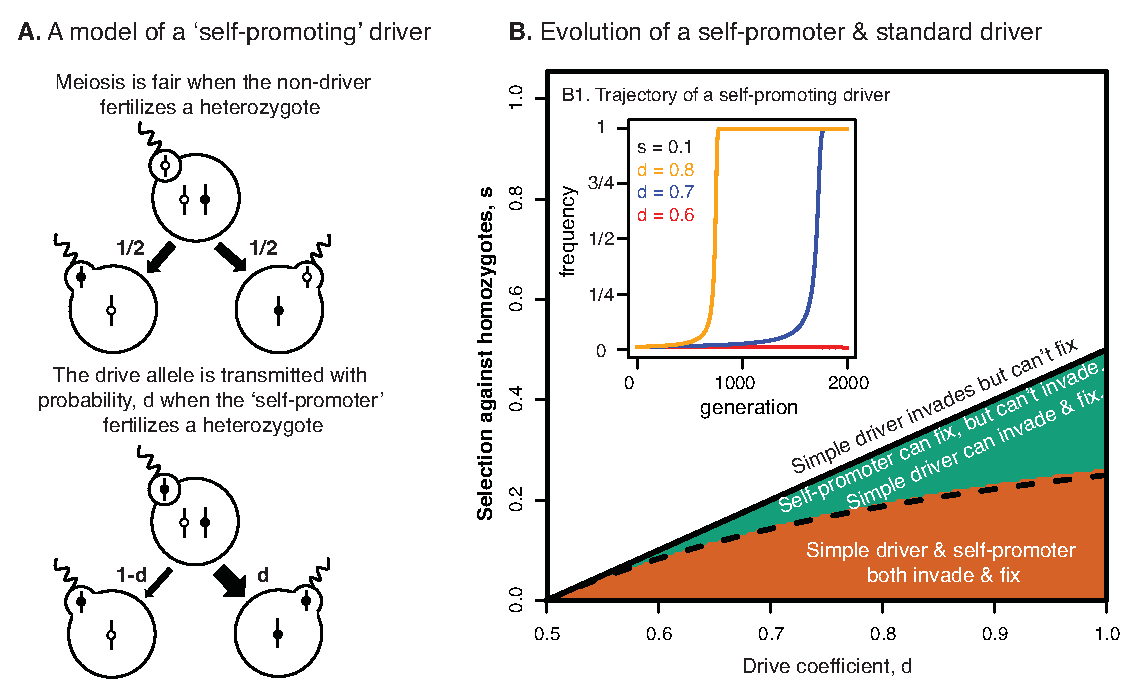
\includegraphics{selfprom.eps}
\caption{{\bf{A.}} A visual depiction of our model of `self-promoting' driver. 
	Transmission probabilities for alleles through female
 	 meiosis depend on sperm genotype. 
	 The non-driving $A$-allele, and self-promoting $B$-allele
	 are represented by unfilled and filled circles, respectively. 
	 {\bf{B.}} Evolution of a self-promoter and standard driver. 
	 	Assuming that the fitnesses of drive homozygotes and 
		heterozygotes are $1-s$ and $1$, respectively. 
	 	\emph{Main figure:} Boundary conditions for the invasion 
		and fixation of self-promoting and standard meiotic drivers, 
		with drive coefficient, $d$. Colored regions depict exact results, 
		while lines  represent analytical approximations. 
	 \emph{B1:}  Trajectories of sperm-dependent female drive
		 %alleles that can invade the population, 
		 each allele has $s =0.1$ against the
		 homozygotes.  The drive coefficient is denoted by color. 
 }   
\label{Eggsperm}
\end{figure*}


\begin{figure*}
	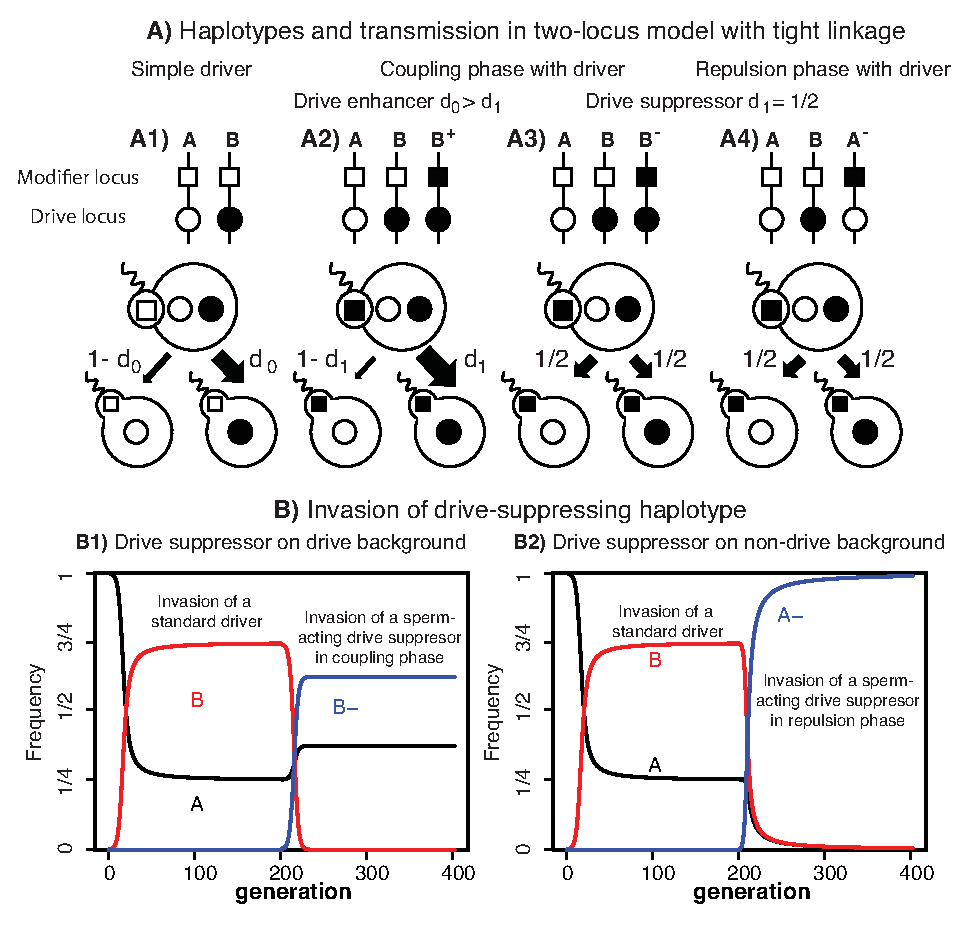
\includegraphics[width = .95
          \textwidth]{twolocus.pdf} 
\caption{Models of a sperm-acting drive modifier tightly linked to a meiotic driver. 
{\bf (A) } 
Sperm carrying the derived allele at the modifier locus (filled squares) alters transmission  
	at the driving allele (filled circles) during female meiosis.
        Alleles at these two tightly linked loci form three haplotypes (top of A). 	
	{\bf{A1)}} In the standard model of drive there is no
        variation at the modifier, 
	and the driver is transmitted to the egg with probability $d_0$. 
	{\bf{A2)}} The modifier allele increases the transmission of the drive allele ($d_1 > d_0$), and due to their shared genetic background, also increases its drive. 
	{\bf{A3 \& A4)}} The sperm-acting modifier acts to decrease
        drive  ($d_1=1/2$ in A3 \& A4, or more generally, $d_1 < d_0$) and arises on the same or opposite
        background from the driver (A3 \& A4 respectively). 
{\bf{(B)}} Invasion of a sperm-acting drive suppressor linked to a driver. 
	After the driver ($B$ haplotype) reaches drive selection equilibrium, we introduce a sperm acting drive modifier. 
	We assume full drive ($D_0 =1$), a recessive lethal fitness cost to drive ($h_s=0$, $s=1$) and that the sperm-acting modifier results in a fair meiosis. 
{\bf {B1)}} The $B^-$ allele replaces the ancestral drive haplotype, but segregates at a lower equilibrium frequency.
{\bf {B2)}} The $A^-$ allele replaces the ancestral non-driving haplotype, and in this case, removes the driver from the population. }
 \label{Eggsperm_3_allele_cartoon}
\end{figure*}


\end{document}

Figure 1 {Eggsperm}
Figure 2 {Eggsperm_3_allele_cartoon}
Figure S1 {Bistab_homozyg_cost_fig}
Figure S2 {bistable_additive}
Figure S3 {Effect_of_dominance}
\end{article}

\begin{figure*}
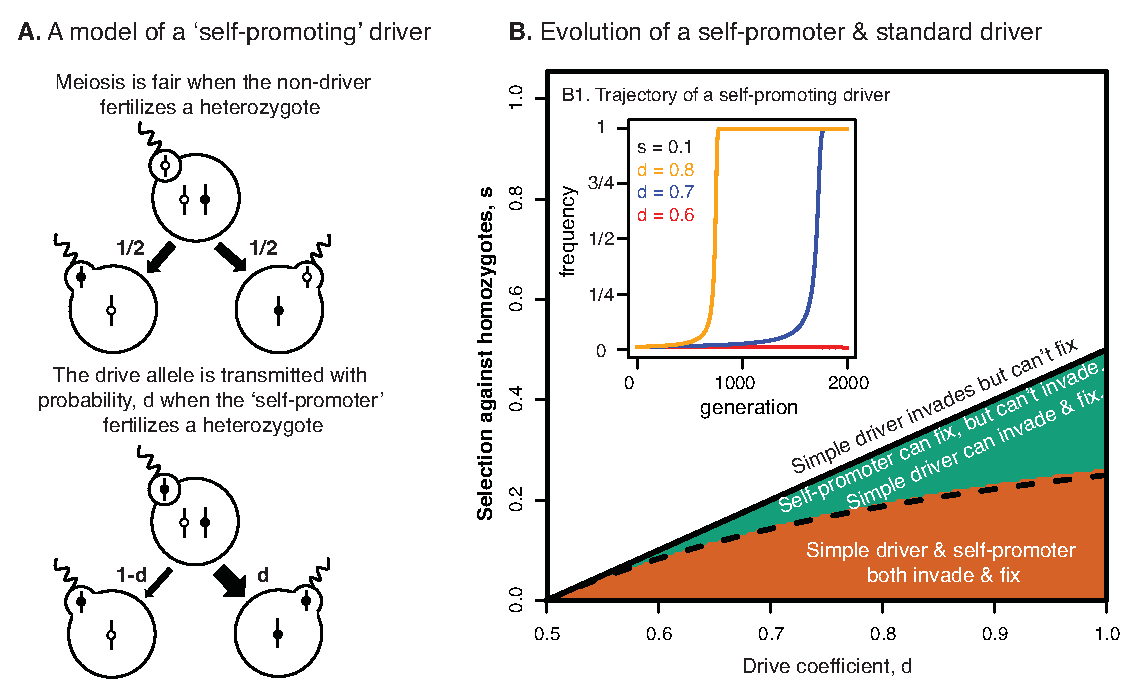
\includegraphics{selfprom.eps}
\caption{{\bf{A.}} A visual depiction of our model of `self-promoting' driver. 
	Transmission probabilities for alleles through female
 	 meiosis depend on sperm genotype. 
	 The non-driving $A$-allele, and self-promoting $B$-allele
	 are represented by unfilled and filled circles, respectively. 
	 {\bf{B.}} Evolution of a self-promoter and standard driver. 
	 	Assuming that the fitnesses of drive homozygotes and 
		heterozygotes are $1-s$ and $1$, respectively. 
	 	\emph{Main figure:} Boundary conditions for the invasion 
		and fixation of self-promoting and standard meiotic drivers, 
		with drive coefficient, $d$. Colored regions depict exact results, 
		while lines  represent analytical approximations. 
	 \emph{B1:}  Trajectories of sperm-dependent female drive
		 %alleles that can invade the population, 
		 each allele has $s =0.1$ against the
		 homozygotes.  The drive coefficient is denoted by color. 
 }   
\label{Eggsperm}
\end{figure*}


\begin{figure*}
	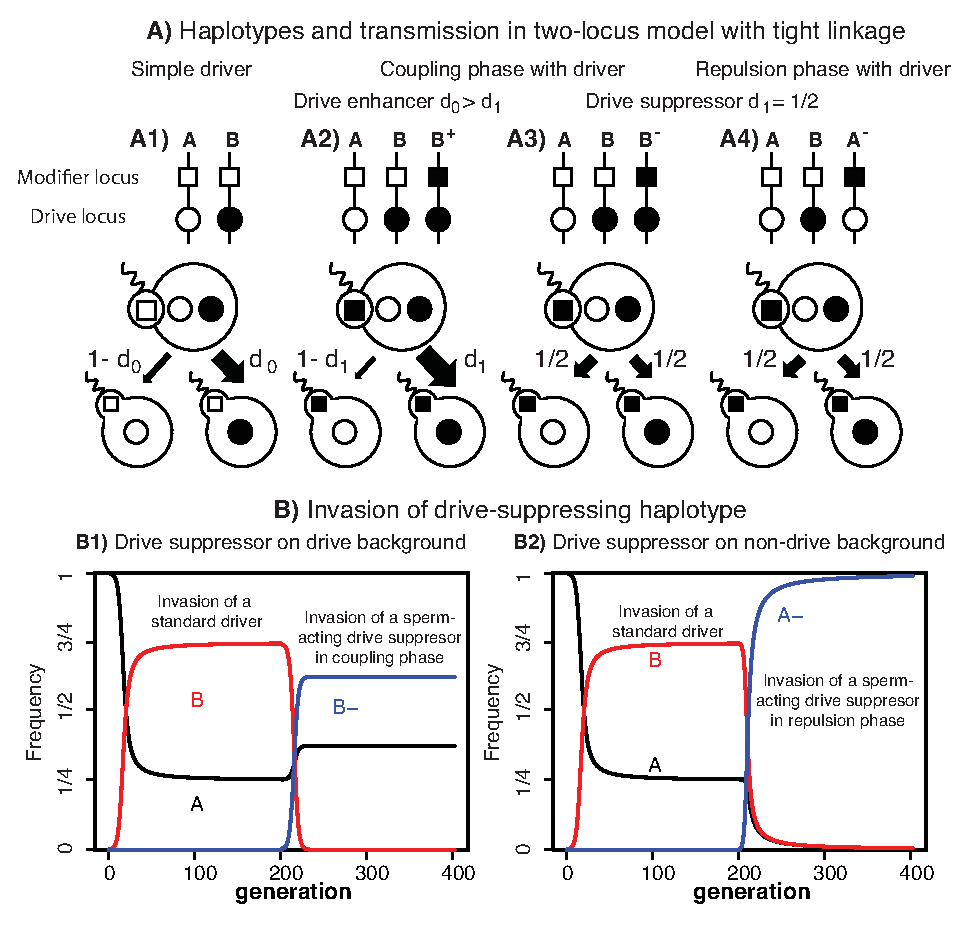
\includegraphics[width = .95
          \textwidth]{twolocus.pdf} 
\caption{Models of a sperm-acting drive modifier tightly linked to a meiotic driver. 
{\bf (A) } 
Sperm carrying the derived allele at the modifier locus (filled squares) alters transmission  
	at the driving allele (filled circles) during female meiosis.
        Alleles at these two tightly linked loci form three haplotypes (top of A). 	
	{\bf{A1)}} In the standard model of drive there is no
        variation at the modifier, 
	and the driver is transmitted to the egg with probability $d_0$. 
	{\bf{A2)}} The modifier allele increases the transmission of the drive allele ($d_1 > d_0$), and due to their shared genetic background, also increases its drive. 
	{\bf{A3 \& A4)}} The sperm-acting modifier acts to decrease
        drive  ($d_1=1/2$ in A3 \& A4, or more generally, $d_1 < d_0$) and arises on the same or opposite
        background from the driver (A3 \& A4 respectively). 
{\bf{(B)}} Invasion of a sperm-acting drive suppressor linked to a driver. 
	After the driver ($B$ haplotype) reaches drive selection equilibrium, we introduce a sperm acting drive modifier. 
	We assume full drive ($D_0 =1$), a recessive lethal fitness cost to drive ($h_s=0$, $s=1$) and that the sperm-acting modifier results in a fair meiosis. 
{\bf {B1)}} The $B^-$ allele replaces the ancestral drive haplotype, but segregates at a lower equilibrium frequency.
{\bf {B2)}} The $A^-$ allele replaces the ancestral non-driving haplotype, and in this case, removes the driver from the population. }
 \label{Eggsperm_3_allele_cartoon}
\end{figure*}


\end{document}

Figure 1 {Eggsperm}
Figure 2 {Eggsperm_3_allele_cartoon}
Figure S1 {Bistab_homozyg_cost_fig}
Figure S2 {bistable_additive}
Figure S3 {Effect_of_dominance}
\end{article}

\begin{figure*}
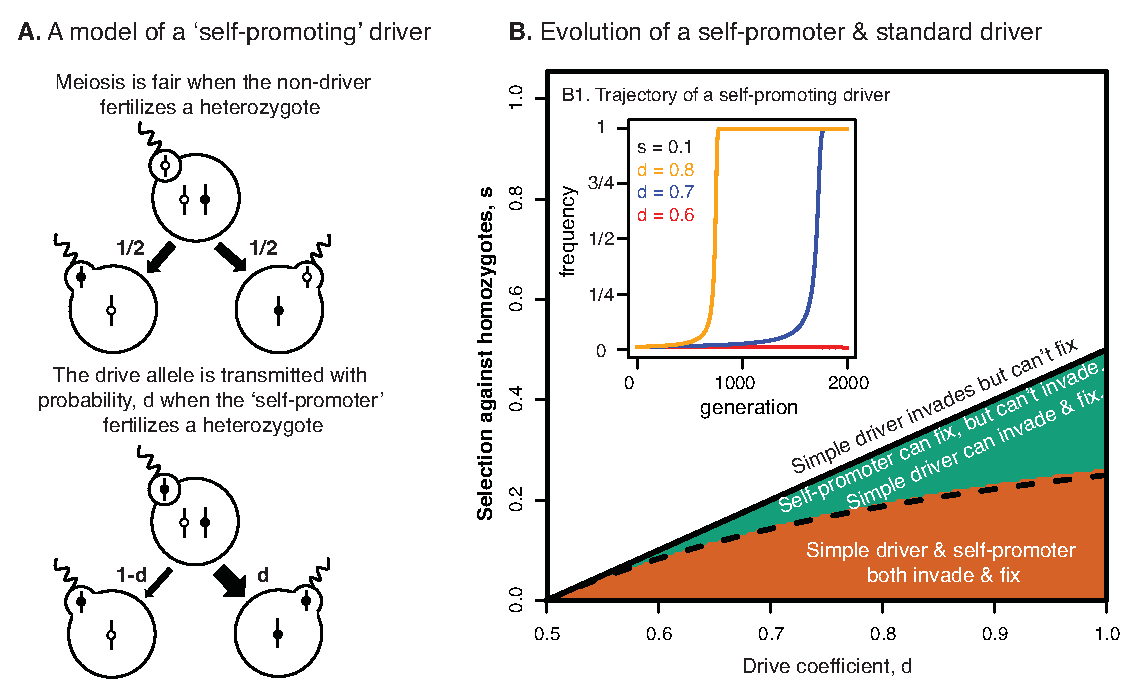
\includegraphics{selfprom.eps}
\caption{{\bf{A.}} A visual depiction of our model of `self-promoting' driver. 
	Transmission probabilities for alleles through female
 	 meiosis depend on sperm genotype. 
	 The non-driving $A$-allele, and self-promoting $B$-allele
	 are represented by unfilled and filled circles, respectively. 
	 {\bf{B.}} Evolution of a self-promoter and standard driver. 
	 	Assuming that the fitnesses of drive homozygotes and 
		heterozygotes are $1-s$ and $1$, respectively. 
	 	\emph{Main figure:} Boundary conditions for the invasion 
		and fixation of self-promoting and standard meiotic drivers, 
		with drive coefficient, $d$. Colored regions depict exact results, 
		while lines  represent analytical approximations. 
	 \emph{B1:}  Trajectories of sperm-dependent female drive
		 %alleles that can invade the population, 
		 each allele has $s =0.1$ against the
		 homozygotes.  The drive coefficient is denoted by color. 
 }   
\label{Eggsperm}
\end{figure*}


\begin{figure*}
	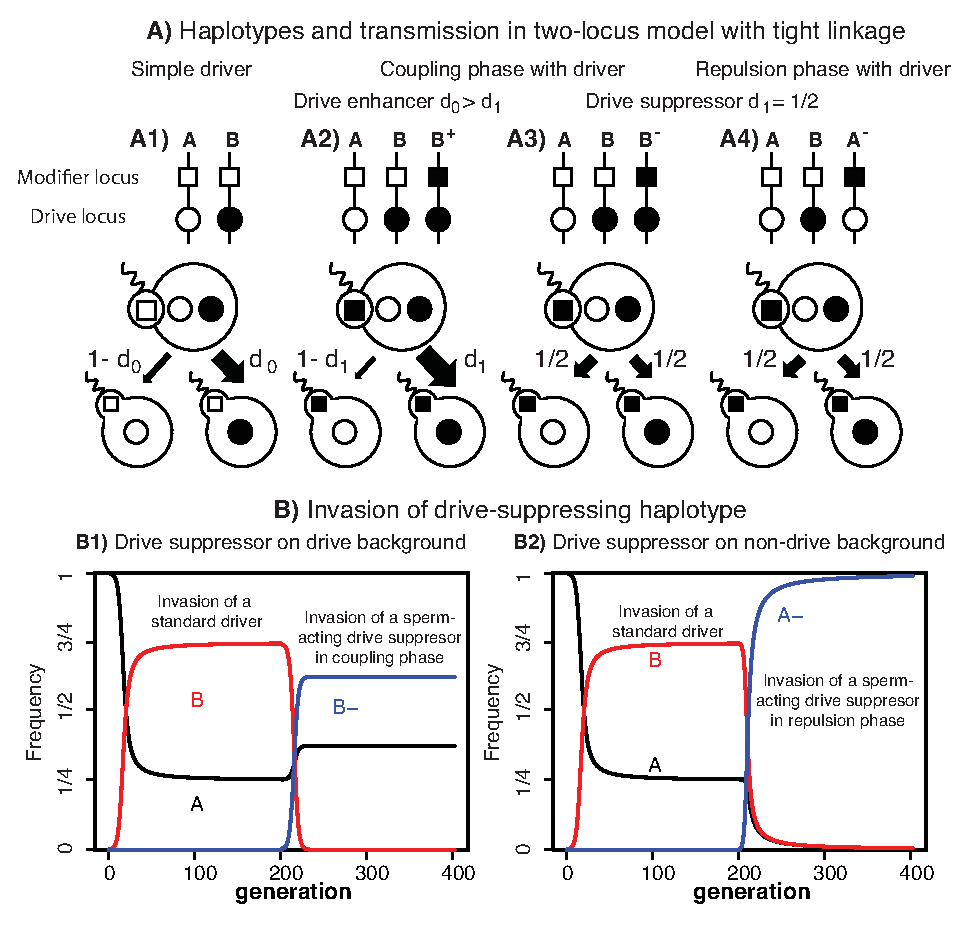
\includegraphics[width = .95
          \textwidth]{twolocus.pdf} 
\caption{Models of a sperm-acting drive modifier tightly linked to a meiotic driver. 
{\bf (A) } 
Sperm carrying the derived allele at the modifier locus (filled squares) alters transmission  
	at the driving allele (filled circles) during female meiosis.
        Alleles at these two tightly linked loci form three haplotypes (top of A). 	
	{\bf{A1)}} In the standard model of drive there is no
        variation at the modifier, 
	and the driver is transmitted to the egg with probability $d_0$. 
	{\bf{A2)}} The modifier allele increases the transmission of the drive allele ($d_1 > d_0$), and due to their shared genetic background, also increases its drive. 
	{\bf{A3 \& A4)}} The sperm-acting modifier acts to decrease
        drive  ($d_1=1/2$ in A3 \& A4, or more generally, $d_1 < d_0$) and arises on the same or opposite
        background from the driver (A3 \& A4 respectively). 
{\bf{(B)}} Invasion of a sperm-acting drive suppressor linked to a driver. 
	After the driver ($B$ haplotype) reaches drive selection equilibrium, we introduce a sperm acting drive modifier. 
	We assume full drive ($D_0 =1$), a recessive lethal fitness cost to drive ($h_s=0$, $s=1$) and that the sperm-acting modifier results in a fair meiosis. 
{\bf {B1)}} The $B^-$ allele replaces the ancestral drive haplotype, but segregates at a lower equilibrium frequency.
{\bf {B2)}} The $A^-$ allele replaces the ancestral non-driving haplotype, and in this case, removes the driver from the population. }
 \label{Eggsperm_3_allele_cartoon}
\end{figure*}


\end{document}

Figure 1 {Eggsperm}
Figure 2 {Eggsperm_3_allele_cartoon}
Figure S1 {Bistab_homozyg_cost_fig}
Figure S2 {bistable_additive}
Figure S3 {Effect_of_dominance}
\end{article}

\begin{figure*}
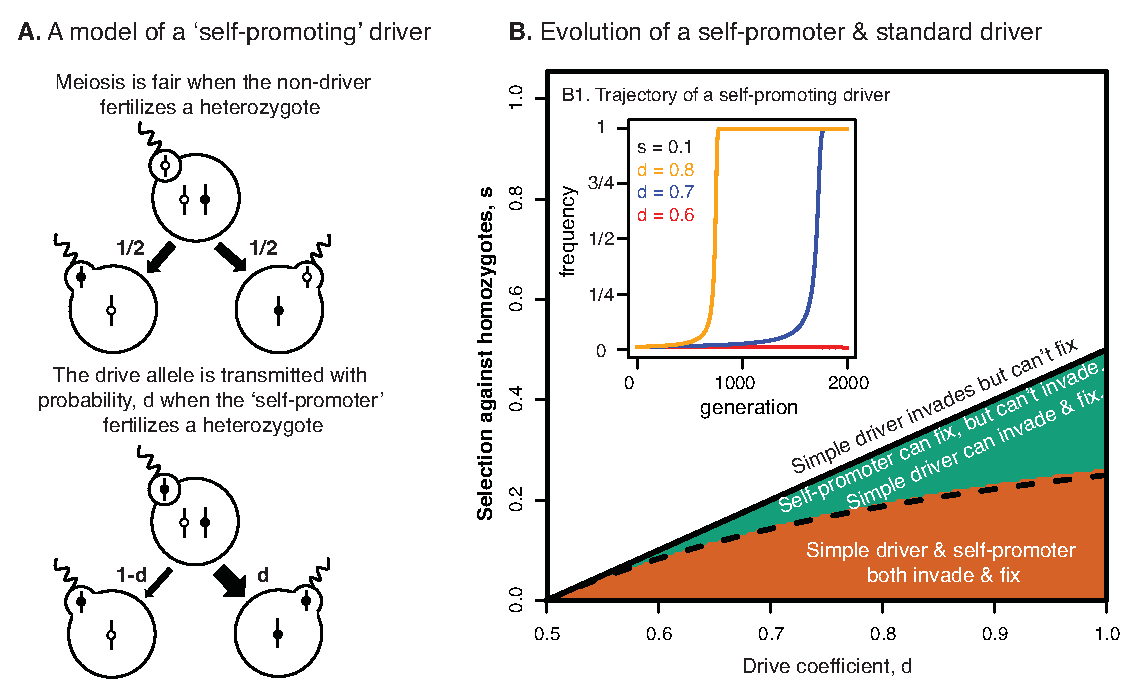
\includegraphics{selfprom.eps}
\caption{{\bf{A.}} A visual depiction of our model of `self-promoting' driver. 
	Transmission probabilities for alleles through female
 	 meiosis depend on sperm genotype. 
	 The non-driving $A$-allele, and self-promoting $B$-allele
	 are represented by unfilled and filled circles, respectively. 
	 {\bf{B.}} Evolution of a self-promoter and standard driver. 
	 	Assuming that the fitnesses of drive homozygotes and 
		heterozygotes are $1-s$ and $1$, respectively. 
	 	\emph{Main figure:} Boundary conditions for the invasion 
		and fixation of self-promoting and standard meiotic drivers, 
		with drive coefficient, $d$. Colored regions depict exact results, 
		while lines  represent analytical approximations. 
	 \emph{B1:}  Trajectories of sperm-dependent female drive
		 %alleles that can invade the population, 
		 each allele has $s =0.1$ against the
		 homozygotes.  The drive coefficient is denoted by color. 
 }   
\label{Eggsperm}
\end{figure*}


\begin{figure*}
	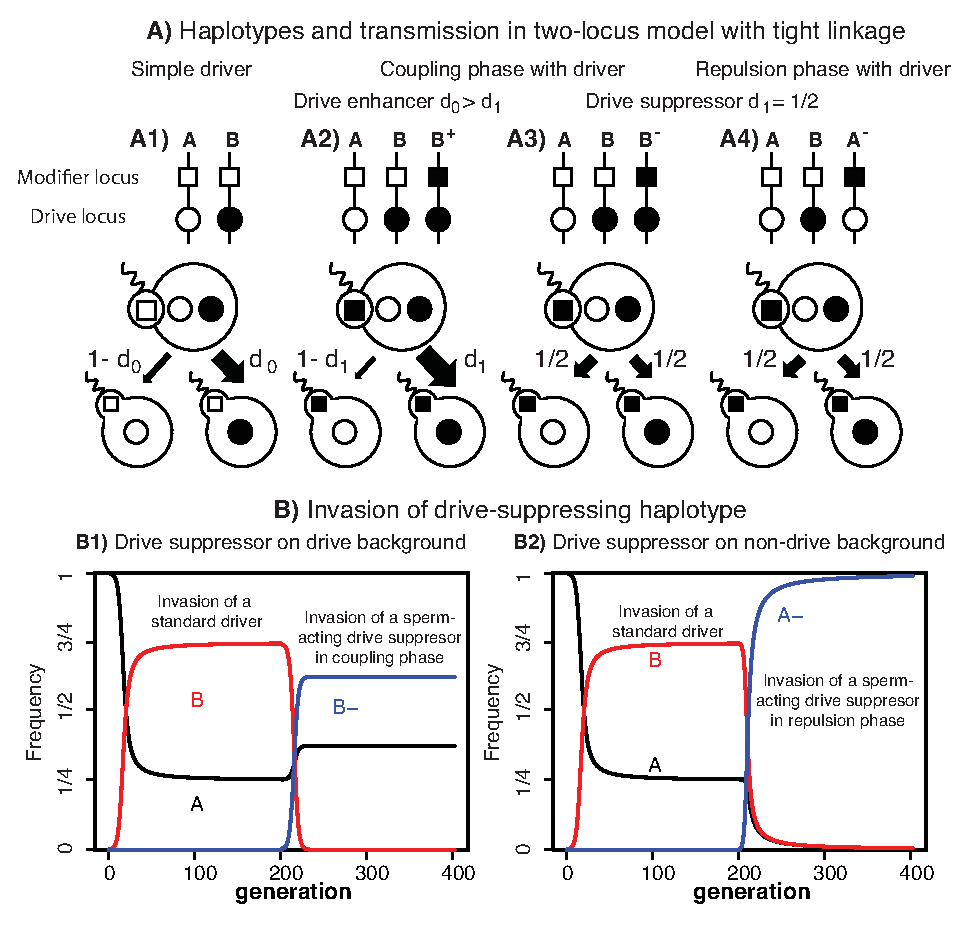
\includegraphics[width = .95
          \textwidth]{twolocus.pdf} 
\caption{Models of a sperm-acting drive modifier tightly linked to a meiotic driver. 
{\bf (A) } 
Sperm carrying the derived allele at the modifier locus (filled squares) alters transmission  
	at the driving allele (filled circles) during female meiosis.
        Alleles at these two tightly linked loci form three haplotypes (top of A). 	
	{\bf{A1)}} In the standard model of drive there is no
        variation at the modifier, 
	and the driver is transmitted to the egg with probability $d_0$. 
	{\bf{A2)}} The modifier allele increases the transmission of the drive allele ($d_1 > d_0$), and due to their shared genetic background, also increases its drive. 
	{\bf{A3 \& A4)}} The sperm-acting modifier acts to decrease
        drive  ($d_1=1/2$ in A3 \& A4, or more generally, $d_1 < d_0$) and arises on the same or opposite
        background from the driver (A3 \& A4 respectively). 
{\bf{(B)}} Invasion of a sperm-acting drive suppressor linked to a driver. 
	After the driver ($B$ haplotype) reaches drive selection equilibrium, we introduce a sperm acting drive modifier. 
	We assume full drive ($D_0 =1$), a recessive lethal fitness cost to drive ($h_s=0$, $s=1$) and that the sperm-acting modifier results in a fair meiosis. 
{\bf {B1)}} The $B^-$ allele replaces the ancestral drive haplotype, but segregates at a lower equilibrium frequency.
{\bf {B2)}} The $A^-$ allele replaces the ancestral non-driving haplotype, and in this case, removes the driver from the population. }
 \label{Eggsperm_3_allele_cartoon}
\end{figure*}


\end{document}

Figure 1 {Eggsperm}
Figure 2 {Eggsperm_3_allele_cartoon}
Figure S1 {Bistab_homozyg_cost_fig}
Figure S2 {bistable_additive}
Figure S3 {Effect_of_dominance}